%! TEX root = ../main.tex

\chapter[Proximal inference based on mixtures of linear models]{Proximal inference based on mixtures of linear models}
\chaptermark{Proximal inference: mixtures of linear models}

% Independence notation (local to this chapter)
\newcommand{\independent}{\protect\mathpalette{\protect\independenT}{\perp}}
\def\independenT#1#2{\mathrel{\rlap{$#1#2$}\mkern2mu{#1#2}}}

\section{Introduction}

In causal inference using observational data, a frequent assumption is that there is no unmeasured confounding. This means that the available covariates are informative enough to ensure that individuals within each stratum of the covariates are comparable across different treatment groups. However, this assumption is often met with doubt, as it requires researchers to accurately capture all relevant confounders, which is rarely achievable in practice. Confounding mechanisms are not always fully identifiable from the measured covariates, meaning that these variables may only serve as imperfect representations of the true confounders. 

\begin{figure}[H]
    \centering
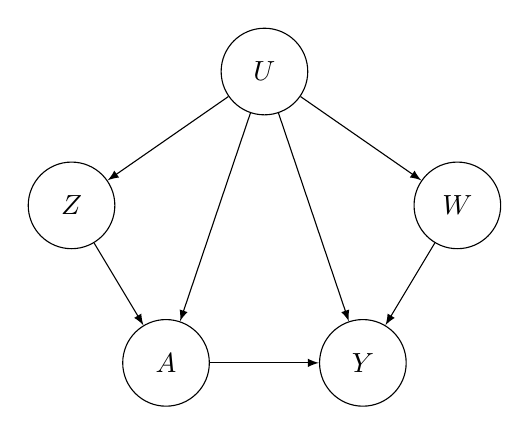
\begin{tikzpicture}[state/.style={circle, draw, minimum size=1.1cm}]
  \def\Ax{0}
  \def\Ay{0}
  \def\offset{2.5}
  \def\Bx{\Ax+5}
  \def\By{\Ay}
  \node[state,shape=circle,draw=black] (Z) at (\Bx-3.7,\Ay+2) {$Z$};
  \node[state,shape=circle,draw=black] (Y) at (\Bx,\By) {$Y$};
  \node[state,shape=circle,draw=black] (A) at (\Bx-2.5,\By) {$A$};
  %\node[state,shape=circle,draw=black] (S) at (\Bx-1.25,\By+1.3) {$S$};
    \node[state,shape=circle,draw=black] (U) at (\Bx-1.25,\By+3.7) {$U$};
  \node[state,shape=circle,draw=black] (W) at (\Bx+1.2,\Ay+2) {$W$};

  %\draw [-latex] (A) to [bend left=0] (W);
  \draw [-latex] (A) to [bend left=0] (Y);
  %\draw [-latex] (A) to [bend left=0] (S);
  %\draw [-latex] (Z) to [bend left=0] (S);
  %\draw [-latex] (A) to [bend left=0] (A);
  %\draw [-latex] (A) to [bend left=0] (Z);
  %\draw [-latex] (S) to [bend left=0] (Y);
  \draw [-latex] (Z) to [bend left=0] (A);
 % \draw [latex-latex] (Z) to [bend left=-35] (A);
  \draw [-latex] (W) to [bend left=0] (Y);
 % \draw [latex-latex] (W) to [bend left=35] (Y);

  \draw [-latex] (U) to [bend left=0] (A);
  \draw [-latex] (U) to [bend left=0] (Z);
  \draw [-latex] (U) to [bend left=0] (Y);
  \draw [-latex] (U) to [bend left=0] (W);
  %\draw [-latex] (U) to [bend left=0] (A);

\end{tikzpicture}
\caption{A Directed Acyclic Graph (DAG) for the classical setting of proximal inference.}
    \label{fig:figure1.0}
\end{figure}

Proximal inference is a method used to uncover treatment effects when standard methods fall short due to unobserved confounders. The key idea of this method is to leverage auxiliary data, the so called \textit{proxy variables}, which carry enough information about the unobserved confounding factors to allow for the estimation of treatment effects. Negative control exposure (NCE) and negative control outcome (NCO) variables are examples of auxiliary data used in this context. An NCO variable $Z$ is a variable known not to be
causally affected by an exposure $A$ and an NCE variable $W$ is a variable known not to cause an outcome $Y$. See Figure \ref{fig:figure1.0} for a typical graph that shows the relations of the proxy variables with the other variables ($U$ contains the unobserved confounders). 

There has been a surge in research on formal methods in proximal inference (see \cite{203,204,205,206,111}). These methods typically depend on assumptions like linear models for outcomes and unmeasured confounders (see \cite{112,113,114,115}), rank preservation (see \cite{116}), monotonicity (see \cite{117}), or categorical unmeasured confounders (see \cite{206}) to identify treatment effects. In \cite{205} and \cite{120} significant contributions were made by presenting conditions for nonparametric identification of treatment effects using treatment and outcome proxies within point treatment contexts.

The method they present relies on the existence of a \textit{bridge function} that connects the observed data. This function, denoted as $(a, w) \mapsto h_{a}(w)$, must satisfy the following relationship for each $A = a$:
\begin{align}\label{eq: bridge function}
    \ex (Y \mid Z, A=a)=\ex \left(h_{a}(W) \mid Z, A=a\right) \quad \quad Z-\text{a.s.}
\end{align}
Under \eqref{eq: bridge function} and the following additional assumptions:
\begin{enumerate}[label=\Alph*.]
    \item $Y(a)=Y$ if $A=a$, \label{ass 1.0} 
    \item $(Y(a),W) \independent (A,Z)\mid U$, \label{ass 2.0}
    \item For any set $\mathfrak{Z}$ with $\pb(Z \in \mathfrak{Z}) = 1$, the set of conditional distributions $\{ \mathcal{L}(U \mid Z=z, A=a) \, : \, z \in \mathfrak{Z} \}$ is complete, \label{ass 3.0}
\end{enumerate}
the average treatment effect of setting $A$ to $a$ is $\ex \, Y(a) = \ex \, h_{a}(W)$. Note that condition \ref{ass 2.0} implies $Y(a) \independent A \mid U$, $Y \independent Z \mid A,U$ and $W \independent (A,Z) \mid U$. The average treatment effect $\ex\, Y(a)$ can be estimated from observational data, without needing direct information about the unmeasured confounder $U$, if the function $h_a$ is known. One of the greatest challenges of the approach based on bridge functions lies in finding the function $h_a$. In the machine learning literature adversarial methods have been developed to estimate $h_a$ from the data (see \cite{118,119}). However in many cases the existence of such function is not clear. A simple setting in which the existence of a bridge function is guaranteed is under the assumptions of linear models for outcomes and unmeasured confounders (see \cite{112,113,114,115}). However this model is too simple to handle most of the applications.

In this chapter, we make two key contributions. First,  we introduce a causal model based on mixtures of linear models for the regression of the outcome $Y$ on the unmeasured confounders and on the covariates. This approach offers flexibility in modeling the distribution of the outcome $Y$ given the covariates $A$ and $Z$. Importantly, we prove that this extension allows the treatment effect to be identifiable, meaning we can derive a closed-form expression for the bridge function $h_a$. Second, we propose a Bayesian nonparametric estimation method. This method models the distribution of the outcome given the covariates using a probit stick-breaking process, with mixing weights that depend on the covariates. We also prove that our methodology is consistent across a range of true underlying causal models. The key advantage of our approach is that it eliminates concerns about the existence of the bridge function $h_a$, as we demonstrate that such a function in this context exists and has an explicit form. However, a limitation of our method is that we still rely on the assumptions of a simpler linear model for the distribution of $W$ given the covariates $A$ and $Z$.

The structure of the chapter is as follows: In Section \ref{sec: mixture of normals}, we begin by revisiting the classical linear model (see \cite{112,113,114,115}) to provide a solid foundation for understanding our extension to mixtures of linear models. We then introduce our proposed model, along with a submodel that utilizes simplified mixing weights. In Section \ref{sec: estimation}, we present the Bayesian nonparametric estimation procedure based on a dependent stick-breaking process and demonstrate that it achieves consistency for a range of underlying causal models.


\section{Mixture of linear models}\label{sec: mixture of normals}

\subsection*{\textit{The classical linear model.}}

One simple case where the form of $h_a$ is known is if we use the restrictive assumption of linear models for the regressions of $Y$ and $W$ on the variables $A,U,Z$ and of $U$ on $A$ and $Z$:
\begin{align*}
    \ex(Y \mid A,U,Z) &= \beta_{0}^{y} + \beta_{1}^{y} A + \beta_{2}^{y} U \numberthis \label{eq: 1a.0}\\
    \ex(W \mid A,U,Z) &= \beta_{0}^{w} + \beta_{1}^{w} U \numberthis \label{eq: 1b.0} \\
    \ex(U \mid A,Z) &= \beta_0^u + \beta_1^u A + \beta_2^u Z \numberthis \label{eq: 3.0}
\end{align*}
By taking conditional expectations given $A,Z$ across the two equations and after some 
algebra (provided that $\beta_1^w \neq 0$), we can obtain the bridge function $h_a$ as:
$$ 
\ex (Y \mid A,Z) = \ex( \beta^y_0 - \beta_2^y\beta^w_0/\beta_1^w + \beta_1^y A + \beta^y_2/\beta_1^w W \mid A,Z).
$$
In the display above we can read out the form of $h_a$ and $\ex \, Y(a+1) - \ex \, Y(a) = \beta_1^y$. 

Since \eqref{eq: 1a.0}-\eqref{eq: 3.0} ensure that the regressions of $Y$ on $A,Z$ and of $W$ on $A,Z$ are linear, there exist coefficients $\theta_{i}^{y}$, $\theta_{i}^{w}$ for $i=1,2,3$:
\begin{align*}
    \ex(Y \mid A,Z) &= \theta_{0}^{y} + \theta_{1}^{y} A + \theta_{2}^{y} Z, \numberthis \label{eq: 1a.0 fit}\\
    \ex(W \mid A,Z) &= \theta_{0}^{w} + \theta_{1}^{w} A + \theta_{2}^{w}  Z, \numberthis \label{eq: 1b.0 fit}
\end{align*}
and we can obtain after some algebra (if $\theta_{2}^{w} \neq 0$, thus $\beta_2^u \neq 0$) that the average treatment effect is given by: 
$$\beta_1^y = \theta_{1}^{y} - \theta_{2}^{y}\theta_{1}^{w}/\theta_{2}^{w}.$$

Note that within this model, the assumptions \eqref{eq: 1a.0}-\eqref{eq: 3.0} remove the need of the completeness assumption of the law of $\mathcal{L}(U \mid Z,A=a)$. It is easy to show that if instead of \eqref{eq: 1a.0}-\eqref{eq: 3.0} we assume the completeness of the law of $\mathcal{L}(U \mid Z,A=a)$ (which intuitively tells that $Z$ must be sufficiently informative about $U$) with \ref{ass 1.0}-\ref{ass 3.0} and that the regressions of $Y$ and $W$ on $A,Z$ are linear as in \eqref{eq: 1a.0 fit}-\eqref{eq: 1b.0 fit}, with $\theta_{2}^{w} \neq 0$, then we can also obtain $h_a$ and thus $\ex \, Y(a)$. 

Although this model is mathematically intriguing because it offers a closed-form example of a bridge function, its reliance on linearity assumptions renders it unsuitable for many scenarios. In the following subsection we will introduce a generalization of this model based on mixture of normals and we will show that it is suitable for a much larger class of underlying models. This model will also provide a closed form expression for the bridge function $h_a$. 

\subsection*{\textit{Extension 1 of the linear model.}}

\emph{The underlying model.} We retain the classical proximal DAG of Figure \ref{fig:figure1.0} and the linear regressions \eqref{eq: 1b.0}-\eqref{eq: 3.0} of the proxy $W$ and of the confounder $U$, but we relax the linearity of the outcome regression \eqref{eq: 1a.0} to
\[
\ex(Y \mid A,U,Z) = f_0(A) + f_2(A)\, U,
\]
for arbitrary measurable functions $f_0, f_2$: the dependence on the exposure is now unrestricted, and only linearity in the unobserved confounder is kept (the latter cannot be relaxed; see Remark \ref{remark: no nonlinear U}).

\emph{The working model.} The underlying model leaves $f_0,f_2$ in $\ex(Y\mid A,U,Z)=f_0(A)+f_2(A)U$ entirely free as functions of $A$. We approximate this regression function by letting the coefficients of the classical linear model vary across a discrete latent \textit{stratum}: a latent variable $S$, drawn given $A$ alone, indexes a family of classical models for the outcome,
\begin{align}\label{eq: model within stratum}
\ex(Y \mid A,U,S) = \beta_{0,S}^{y} + \beta_{1,S}^{y} A + \beta_{2,S}^{y} U,
\end{align}
while $W$ and $U$ keep the unstratified regressions \eqref{eq: 1b.0}--\eqref{eq: 3.0}, i.e.\ $S$ enters the outcome mechanism only. The DAG of Figure~\ref{fig:figure2} displays this construction.
\begin{figure}[H]
\centering

\begin{subfigure}[t]{0.48\textwidth}
\centering
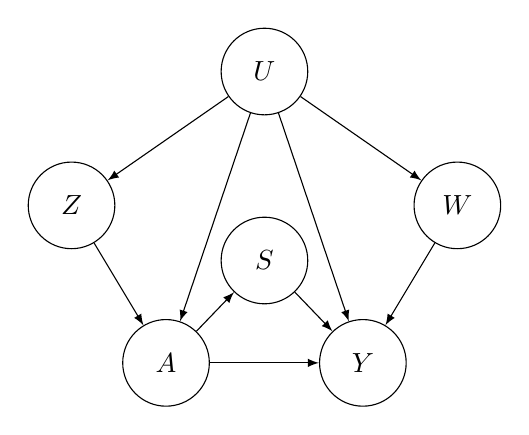
\begin{tikzpicture}[state/.style={circle, draw, minimum size=1.1cm}]
  \def\Ax{0}
  \def\Ay{0}
  \def\offset{2.5}
  \def\Bx{\Ax+5}
  \def\By{\Ay}
  \node[state,shape=circle,draw=black] (Z) at (\Bx-3.7,\Ay+2) {$Z$};
  \node[state,shape=circle,draw=black] (Y) at (\Bx,\By) {$Y$};
  \node[state,shape=circle,draw=black] (A) at (\Bx-2.5,\By) {$A$};
  \node[state,shape=circle,draw=black] (S) at (\Bx-1.25,\By+1.3) {$S$};
  \node[state,shape=circle,draw=black] (U) at (\Bx-1.25,\By+3.7) {$U$};
  \node[state,shape=circle,draw=black] (W) at (\Bx+1.2,\Ay+2) {$W$};

  \draw [-latex] (A) to [bend left=0] (Y);
  \draw [-latex] (A) to [bend left=0] (S);
  \draw [-latex] (S) to [bend left=0] (Y);
  \draw [-latex] (Z) to [bend left=0] (A);
  \draw [-latex] (W) to [bend left=0] (Y);

  \draw [-latex] (U) to [bend left=0] (A);
  \draw [-latex] (U) to [bend left=0] (Z);
  \draw [-latex] (U) to [bend left=0] (Y);
  \draw [-latex] (U) to [bend left=0] (W);
\end{tikzpicture}
\caption{DAG with latent node $S$.}
\label{fig:figure2}
\end{subfigure}\hfill
\begin{subfigure}[t]{0.48\textwidth}
\centering
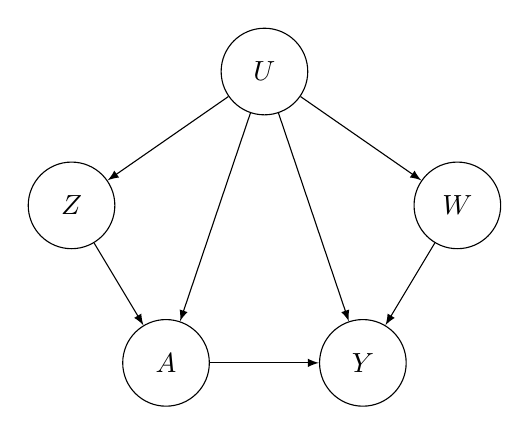
\begin{tikzpicture}[state/.style={circle, draw, minimum size=1.1cm}]
  \def\Ax{0}
  \def\Ay{0}
  \def\offset{2.5}
  \def\Bx{\Ax+5}
  \def\By{\Ay}
  \node[state,shape=circle,draw=black] (Z) at (\Bx-3.7,\Ay+2) {$Z$};
  \node[state,shape=circle,draw=black] (Y) at (\Bx,\By) {$Y$};
  \node[state,shape=circle,draw=black] (A) at (\Bx-2.5,\By) {$A$};
  \node[state,shape=circle,draw=black] (U) at (\Bx-1.25,\By+3.7) {$U$};
  \node[state,shape=circle,draw=black] (W) at (\Bx+1.2,\Ay+2) {$W$};

  \draw [-latex] (A) to [bend left=0] (Y);
  \draw [-latex] (Z) to [bend left=0] (A);
  \draw [-latex] (W) to [bend left=0] (Y);

  \draw [-latex] (U) to [bend left=0] (A);
  \draw [-latex] (U) to [bend left=0] (Z);
  \draw [-latex] (U) to [bend left=0] (Y);
  \draw [-latex] (U) to [bend left=0] (W);
\end{tikzpicture}
\caption{Marginal DAG after integrating out $S$.}
\label{fig:figure2.1}
\end{subfigure}

\caption{Extension 1. \subref{fig:figure2}: the DAG that motivates the shape of the working model, with the latent stratum variable $S$ entering the outcome mechanism; \subref{fig:figure2.1}: its marginalization over $S$, which coincides with the classical proximal DAG of Figure \ref{fig:figure1.0} on which the underlying model is based. The DAG \subref{fig:figure2} is motivation only and is nowhere assumed.}

\end{figure}

Marginalising out $S$ returns the DAG of Figure \ref{fig:figure2.1}, which coincides with the classical proximal DAG of Figure \ref{fig:figure1.0} on which the underlying model is based: the DAG implies $S \independent (W,U,Z) \mid A$ and $Y \independent Z \mid A,U,S$, whence
\[
\ex(Y \mid A,U,Z) = \ex(\beta_{0,S}^{y}\mid A) + \ex(\beta_{1,S}^{y}\mid A)\,A + \ex(\beta_{2,S}^{y}\mid A)\,U,
\]
which is of the underlying form $f_0(A) + f_2(A)U$: as $S$ ranges over strata with weights depending on $A$, the stratum average $A \mapsto \ex(\beta_{2,S}^y \mid A)$ can approximate an arbitrary function of $A$, which is exactly the extra flexibility that the underlying model allows over the classical one. The same independences turn \eqref{eq: model within stratum} into stratum-wise linear regression of the observables,
\[
\ex(Y \mid A,S,Z) = \theta_{0,S}^{y} + \theta_{1,S}^{y} A + \theta_{2,S}^{y} Z, \qquad \ex(W \mid A,Z) = \theta_0^w + \theta_1^w A + \theta_2^w Z,
\]
with $\theta_{i,S}^y$ an explicit affine function of $\beta_{0,S}^y,\beta_{1,S}^y,\beta_{2,S}^y$ and $\theta_i^w$ as in the classical model (the exact substitution is carried out in the remark following the theorem). Averaging over $S \mid A$ turns this into a mixture representation of the observables,
\begin{align*}
    & S \mid A \sim (w_k(A))_{k \in \mathbb{N}} \numberthis \label{eq: weights distr 1} \\
    &Y \mid A, Z \sim \sum_{k =1}^{\infty} w_k (A) \,  N(\theta_{0,k}^{y} + \theta_{1,k}^{y} A + \theta_{2,k}^{y} Z, \sigma^2_{y,k}) \numberthis \label{eq: law of Y|A,Z 1}\\
    & W \mid A,Z \sim N(\theta_{0}^{w} + \theta_{1}^{w} A + \theta_{2}^{w} Z, \sigma^2_{w}), \numberthis \label{eq: law of W|A,Z 1}
\end{align*}
and it is a model of this form --- with $(\theta^y_{i,k})_{i\in\{0,1,2\},k\in\mathbb{N}}$, $(\theta^w_i)_{i\in\{0,1,2\}}$ and $(w_k(A))_{k\in\mathbb{N}}$ now treated as free parameters, rather than fixed at the values determined by the betas above --- that we fit to a sample $(Z,A,Y,W)$ via the Bayesian nonparametric procedure of Section~\ref{sec: estimation}.

The DAG, the latent $S$, and the betas above were introduced only to motivate this particular family of mixtures as working model; nothing about them is assumed of the mechanism that generates the data. What matters instead is a property of the family \eqref{eq: weights distr 1}--\eqref{eq: law of W|A,Z 1} that we call \emph{stratum representation} of the observables. This concept is formalized in part (b) of the theorem below. In essence a \emph{stratum representation} of the observables is an enrichment of the law of $(Z,A,Y,W)$ with a latent variable $S$ that allows us to express the conditional expectation of $Y \mid A, Z$ as a mixture of linear regressions within each strata. Part (a) in the theorem below identifies the ATE of the underlying model by an explicit functional of the laws of the observables, and part (b) shows that every stratum representation collapses this functional into the closed form computed by the fitted working model.


\begin{theorem}[Extension 1]\label{thm: extension 1}\label{lemma: identify EYa from data 1}\label{prop: underlying0_clean}\label{prop: equivalence ATE simpler}
Suppose $(U,Z,A,Y,W)$ follows the underlying model: the DAG of Figure \ref{fig:figure1.0} (hence the consistency \ref{ass 1.0} and the conditional independence \ref{ass 2.0}) and
\begin{enumerate}
\item $\ex(Y \mid A,U,Z) = f_0(A) + f_2(A)U$, for some measurable functions $f_0, f_2$, \label{ass: first ass underlying clean}
\item $\ex(W \mid A,U,Z) = \beta_0^w + \beta_1^w U$, with $\beta_1^w \neq 0$,
\item $\ex(U \mid A,Z) = \beta_0^u + \beta_1^u A + \beta_2^u Z$, with $\beta_2^u \neq 0$,
\end{enumerate}
and fix $a \in \mathcal A$ with $\mathrm{Var}(Z \mid A=a) \in (0,\infty)$. Then:
\begin{enumerate}[label=\textup{(\alph*)}]
\item (Identification) The regressions of the observables are,
\begin{align}
    \ex(Y \mid A=a,Z) &= g_0(a) + g_2(a) Z, \qquad \, \, g_2(a) = f_2(a)\,\beta_2^u, \label{eq: obs Y regression ext1}\\
    \ex(W \mid A,Z) &= \theta_{0}^{w} + \theta_{1}^{w} A  + \theta_{2}^{w} Z, \qquad \theta_2^w = \beta_1^w \beta_2^u \neq 0, \label{eq: 2b.1}
\end{align}
and the ATE is given by
\begin{align}\label{eq: ATE underlying ext1}
\ex \, Y(a)
=
\ex[\ex(Y\mid A=a,Z)]
+
\gamma(a)\,
\ex\!\big[
\ex(W\mid A,Z)-\ex(W\mid A=a,Z)
\big],
\end{align}
where $\gamma(a)$ is identified from the laws of the observables:
\[
\gamma(a) = \frac{\mathrm{Cov}\!\left(Z, \ex(Y\mid A=a,Z)\mid A=a\right)}
{\mathrm{Cov}\!\left(Z, \ex(W\mid A=a,Z)\mid A=a\right)} = \frac{g_2(a)}{\theta_2^w}.
\]
\item (Closed form under a stratum representation) Let $(Z,A,Y,W,S)$ be any stratum representation of the observables: a random vector, on some probability space, whose first four coordinates are distributed as the observables and such that
\begin{align}
        S \independent Z \mid A \qquad \text{and} \qquad \ex(Y \mid A,S,Z) = \theta_{0,S}^{y} + \theta_{1,S}^{y} A + \theta_{2,S}^{y} Z, \label{eq: 2a.1}
\end{align}
for some coefficients $(\theta^y_{i,s})_{i \in \{0,1,2\}, s \in \mathbb{N}}$. Then, for $\boldsymbol{\theta}_i (a) = \ex (\theta_{i,S}^{y} \mid A = a)$,
\[
\frac{\boldsymbol{\theta}_2(a)}{\theta_2^w} = \gamma(a),
\]
and the ATE takes the closed form
    \begin{align}\label{eq: expression for ATE first model}
        \ex \, Y(a)
        &= \ex\,\ex(Y \mid A=a,Z) + \frac{\boldsymbol{\theta}_2(a)}{\theta_2^w}\,\ex\!\big[\ex(W \mid A,Z)-\ex(W \mid A=a,Z)\big] \nonumber\\
        &= \boldsymbol{\theta}_0(a) + \boldsymbol{\theta}_1(a)\,a + \frac{\boldsymbol{\theta}_2(a)}{\theta_2^w}\!\left(\ex W - \theta_0^w - \theta_1^w a\right).
    \end{align}
\end{enumerate}
\end{theorem}

\begin{remark}[A stronger but easier to interpret sufficient condition for part (b)]
The stratum representation condition \eqref{eq: 2a.1} can be replaced by the stronger, more directly interpretable assumption that $S \independent (U,Z) \mid A$ and
\[
\ex(Y \mid A,U,S) = \beta_{0,S}^{y} + \beta_{1,S}^{y} A + \beta_{2,S}^{y} U,
\]
i.e.\ that \eqref{eq: model within stratum} holds within every stratum. Together with assumption~3 of the theorem ($\ex(U\mid A,Z) = \beta_0^u + \beta_1^u A + \beta_2^u Z$), iterated expectation gives
\[
\ex(Y \mid A,S,Z) = (\beta_{0,S}^y + \beta_{2,S}^y\beta_0^u) + (\beta_{1,S}^y + \beta_{2,S}^y\beta_1^u)\,A + \beta_{2,S}^y\beta_2^u\,Z,
\]
which is exactly \eqref{eq: 2a.1} with $\theta_{0,S}^y = \beta_{0,S}^y + \beta_{2,S}^y\beta_0^u$, $\theta_{1,S}^y = \beta_{1,S}^y + \beta_{2,S}^y\beta_1^u$, and $\theta_{2,S}^y = \beta_{2,S}^y\beta_2^u$. This is strictly stronger than \eqref{eq: 2a.1} because it constrains the stratum structure at the level of the unobserved confounder $U$, not merely at the level of the observables. The theorem is stated in the weaker form \eqref{eq: 2a.1} because that is all that is needed.
\end{remark}

\begin{proof}
\emph{Part (a).} Write $m_Y(a,z)=\ex(Y\mid A=a,Z=z)$ and $m_W(a,z)=\ex(W\mid A=a,Z=z)$. By the tower property of conditional expectation,
\begin{align*}
\ex(Y\mid A,Z)
&=f_0(A)+f_2(A)\ex(U\mid A,Z) \\
&=f_0(A)+f_2(A)(\beta_0^u+\beta_1^uA+\beta_2^uZ) =: g_0(A)+g_2(A)Z,
\end{align*}
where $g_2(A)=f_2(A)\beta_2^u$, and $g_0$ collects the remaining terms; this is \eqref{eq: obs Y regression ext1}. Similarly, by iterated expectation,
\[
\ex(W\mid A,Z)=\beta_0^w+\beta_1^w\ex(U\mid A,Z)=\theta_0^w+\theta_1^wA+\theta_2^w Z,
\]
with $\theta_2^w=\beta_1^w\beta_2^u\neq 0$, which is \eqref{eq: 2b.1}.

The slope $g_2(a)$ is identified from the observable regression $m_Y(a,\cdot)$: letting $Q_a$ denote the law of $Z\mid A=a$ and using $\mathrm{Var}(Z\mid A=a)>0$, it admits the explicit form
\begin{align}
g_2(a)
=
\frac{\ex\!\left[(Z-\ex(Z\mid A=a))\,m_Y(a,Z)\mid A=a\right]}
{\mathrm{Var}(Z\mid A=a)}.
\label{eq:g2_projection_formula}
\end{align}
To verify \eqref{eq:g2_projection_formula}, write $m_Y(a,Z)=g_0(a)+g_2(a)Z$ and note that
\begin{align*}
\ex[(Z-\mu_a)m_Y(a,Z)\mid A=a]
&=\ex[(Z-\mu_a)(g_0(a)+g_2(a)Z)\mid A=a] \\
&=g_2(a)\ex[(Z-\mu_a)Z\mid A=a]
=g_2(a)\mathrm{Var}(Z\mid A=a),
\end{align*}
where $\mu_a=\ex(Z\mid A=a)$; dividing by $\mathrm{Var}(Z\mid A=a)$ yields \eqref{eq:g2_projection_formula}.
(If $Z\in\{0,1\}$, this reduces to $g_2(a)=m_Y(a,1)-m_Y(a,0)$.)
In the same way, since $m_W(a,z)=h_0(a)+\theta_2^w z$ for fixed $a$,
\begin{align}
\theta_2^w
=
\frac{\ex\!\left[(Z-\mu_a)\,m_W(a,Z)\mid A=a\right]}
{\mathrm{Var}(Z\mid A=a)}.
\label{eq:theta2w_projection_formula}
\end{align}
Combining \eqref{eq:g2_projection_formula}--\eqref{eq:theta2w_projection_formula} yields
\[
\frac{g_2(a)}{\theta_2^w}
=
\frac{\ex[(Z-\mu_a)m_Y(a,Z)\mid A=a]}{\ex[(Z-\mu_a)m_W(a,Z)\mid A=a]}
=
\frac{\mathrm{Cov}\!\left(Z, m_Y(a,Z)\mid A=a\right)}{\mathrm{Cov}\!\left(Z, m_W(a,Z)\mid A=a\right)}
= \gamma(a),
\]
the denominator being nonzero by $\theta_2^w\neq 0$ and $\mathrm{Var}(Z\mid A=a)>0$.
Finally, using the consistency \ref{ass 1.0} and $Y(a)\independent A\mid(U,Z)$, which is implied by \ref{ass 2.0}, together with the tower property of conditional expectation, we obtain
\begin{align*}
    \ex \, Y(a) &= \ex \big[ \ex (Y(a)\mid A=a,U,Z)\big] = \ex \big[f_0(a) + f_2(a)U\big] = f_0(a) + f_2(a)\ex (U) \\ &= \ex [ \ex (Y\mid A=a,Z)] + f_2(a)\ex \big( \ex (U\mid Z) - \ex (U \mid A=a,Z)\big) \\ &= \ex [ \ex (Y\mid A=a,Z)] + \frac{g_2(a)}{\theta_2^w} \ex \!\left( \ex (W \mid A,Z) - \ex ( W \mid A=a,Z) \right),
\end{align*}
which is \eqref{eq: ATE underlying ext1}.

\emph{Part (b).} A stratum representation leaves the law of the observables unchanged, so every conditional expectation below may be computed on the space carrying it. By $S \independent Z \mid A$ and \eqref{eq: 2a.1},
\[
\ex(Y \mid A=a,Z) = \ex\big(\theta_{0,S}^{y} + \theta_{1,S}^{y}\,a + \theta_{2,S}^{y}\,Z \mid A=a, Z\big) = \boldsymbol{\theta}_0(a) + \boldsymbol{\theta}_1(a)\,a + \boldsymbol{\theta}_2(a)\,Z,
\]
while part (a) gives $\ex(Y \mid A=a,Z) = g_0(a) + g_2(a)Z$. These are two affine representations of the same regression $z \mapsto \ex(Y \mid A=a,Z=z)$: their difference, an affine function of $z$, vanishes for $Q_a$-almost every $z$, and since $\mathrm{Var}(Z \mid A=a)>0$ the law $Q_a$ charges at least two points, so both its coefficients are zero. Whence $\boldsymbol{\theta}_2(a) = g_2(a)$ and $\boldsymbol{\theta}_2(a)/\theta_2^w = g_2(a)/\theta_2^w = \gamma(a)$ by part (a). Substituting into the ATE formula \eqref{eq: ATE underlying ext1} of part (a) and using \eqref{eq: 2b.1},
\begin{align*}
\ex \, Y(a) &= \ex\,\ex(Y \mid A=a,Z) + \frac{\boldsymbol{\theta}_2(a)}{\theta_2^w}\, \ex\big[\ex(W \mid A,Z) - \ex(W \mid A=a,Z)\big] \\
&= \boldsymbol{\theta}_0(a) + \boldsymbol{\theta}_1(a)\,a + \boldsymbol{\theta}_2(a)\,\ex Z + \frac{\boldsymbol{\theta}_2(a)}{\theta_2^w}\,\theta_1^w(\ex A - a),
\end{align*}
and since $\ex W = \theta_0^w + \theta_1^w \ex A + \theta_2^w \ex Z$ by \eqref{eq: 2b.1}, the right-hand side equals $\boldsymbol{\theta}_0 (a) + \boldsymbol{\theta}_1 (a) a + \frac{\boldsymbol{\theta}_2(a)}{\theta_{2}^{w}} (\ex W - \theta_{0}^{w} - \theta_{1}^{w} a)$, which is \eqref{eq: expression for ATE first model}.
\end{proof}

After choosing a prior for $((\theta^y_{i,k})_{k \in \mathbb{N}, i \in \{0,1,2\} }, (\theta^w_{i})_{i \in \{0,1,2\}}, (w_k(A))_{k \in \mathbb{N}})$, any posterior draw of the parameters  of the working model \eqref{eq: weights distr 1}-\eqref{eq: law of W|A,Z 1} carries a stratum representation of the fitted law of the observables: the mixing weights depend on the exposure only, so $S \independent Z \mid A$, and the mixture components are linear, which is \eqref{eq: 2a.1}. With $\boldsymbol{\theta}_i(a) = \sum_{k} w_k(a)\, \theta^y_{i,k}$, the closed form \eqref{eq: expression for ATE first model} of Theorem \ref{thm: extension 1}(b) reads
\begin{align*}
 \ex \, Y(a)&= \sum_{k \geq 1} w_k(a)\left(\theta_{0,k}^{y}+\theta_{1, k}^{y} a-\frac{\theta_{2, k}^{y}}{\theta_2^{w}}\left(\theta_0^{w}+\theta_1^{w} a\right)\right)+\sum_{k=1} \frac{\theta_{2, k}^{y}}{\theta_2^{w}} w_k(a) \ex\left( W\right), \numberthis \label{eq: first formula to rewrite}
\end{align*}
so the posterior on the parameters induces, through \eqref{eq: first formula to rewrite}, a posterior on the ATE. The scope of this procedure is exactly the content of Theorem \ref{thm: extension 1}: the quantity estimated by \eqref{eq: first formula to rewrite} equals $\ex \, Y(a)$ under every underlying model satisfying the assumptions of the theorem, whichever stratum representation the fit selects; in particular, whether or not the working model is correctly specified with respect to the $U$. Moreover, since by part (a) the ATE is a continuous functional of the regressions of the observables, consistent estimation of these regressions translates into consistent estimation of the ATE; this is made precise in Section \ref{sec: estimation}.



\begin{remark}[Linearity in $U$ cannot be dropped]\label{remark: no nonlinear U}
    One may wonder whether it is possible to generalize assumption \ref{ass: first ass underlying clean} of the underlying model class to an expression nonlinear in $U$. We show it is not possible. Consider an underlying model in which, for some $f_0$:
\begin{align*}
    &\ex(Y \mid A, U) = f_0(A,U) \\
    &\ex(W \mid A, U) = \beta^{w}_0 + \beta_1^{w} U \\
    & \ex(U \mid A,Z) = \beta_0^u + \beta_1^u A + \beta_2^u Z,
\end{align*}
therefore we can find $\theta_i^w$ such that $\ex(W \mid A,Z) = \theta_{0}^{w} + \theta_{1}^{w} A + \theta_{2}^{w} Z$. Then $\ex \, Y(a) = \ex f_0(a,U)$ and define $z_a := \frac{1}{\theta_2^{w}} ( \theta_1^{w} (\ex A - a) + \theta_2^{w} \ex Z)$. Then:
\begin{align*}
    &\ex(Y \mid A=a, Z) = \ex ( f_0(a,U) \mid A=a,Z) \\
    &\ex(W \mid A=a, Z= z_a) = \ex W
\end{align*}
on the other hand:
\begin{align*}
    \ex(W \mid A,Z) = \beta^{w}_0 + \beta_1^{w} \ex( U \mid A,Z) \, \implies \, \ex W = \beta^{w}_0 + \beta_1^{w} \ex( U )
\end{align*}
therefore:
\begin{align*}
    \beta^{w}_0 + \beta_1^{w} \ex( U ) = \ex W = \ex (W \mid A=a, Z= z_a) = \beta^{w}_0 + \beta_1^{w} \ex( U \mid A=a, Z= z_a ) 
\end{align*}
which implies: $\ex(U) = \ex(U \mid A=a, Z= z_a)$. Thus in this case the following formula is true only if we can exchange $f_0$ with the expectation, i.e. $f_0$ is linear in $U$ ($f_0(a,U) = f_0(a) + f_2(a) U$):
\begin{align*}
    & \ex( Y \mid A=a, Z= z_a) = \ex( f_0(a,U) \mid A=a, Z= z_a)  \\
    &=  f_0(a) + f_2(a) \ex( U \mid A=a, Z= z_a ) =  f_0(a) + f_2(a) \ex(U) = \ex f_0(a,U) = \ex \, Y(a) 
\end{align*}
\end{remark}



\subsection*{\textit{Extension 2 of the linear model.}}

\emph{The underlying model.} In the second extension we enlarge the class of underlying models by allowing the proxy $Z$ to affect the outcome directly. The underlying model now follows the DAG of Figure \ref{fig:figure1.1}, which augments the classical proximal DAG with the edge $Z \to Y$, and the outcome regression may depend on $Z$ and interact it with the confounder,
\[
\ex(Y\mid A,U,Z)= f_0(A,Z) + \{\alpha_0(A)+\alpha_1(A)Z\}\,U,
\]
while the regressions of $W$ and $U$ keep the same form as before. The DAG encodes the consistency assumption and the conditional independence read from its SWIG,
\begin{multicols}{2}
    \begin{enumerate}
        \item $Y(a)=Y$ if $A=a$ \label{ass 1}
        \item $Y(a) \independent A \mid U,Z$ \label{ass 2}
    \end{enumerate}
\end{multicols}
\noindent Although the DAG of Figure \ref{fig:figure1.1} is not identical to the canonical proximal DAG, it remains proximal in the sense relevant for identification, since proximal assumptions are structural constraints on proxy roles rather than exact graphical equalities: $W$ is still a valid negative-control outcome proxy (it is not causally affected by $A$, and $W \independent (A,Z) \mid U$), $Z$ is still a valid pre-exposure proxy (it does not causally affect $Y$), and both proxies remain informative about the latent confounder $U$, which is the key requirement enabling proximal identification.

\emph{The working model.} As in Extension 1, an outcome regression that interacts $A,Z$ and $U$ through the arbitrary functions $f_0,\alpha_0,\alpha_1$ cannot be fitted directly. We extend the Extension~1 construction by letting the stratum label also depend on the proxy $Z$: a label $S$, drawn given $(A,Z)$, indexes a family of classical models for the outcome as in \eqref{eq: model within stratum},
\[
\ex(Y \mid A,U,S,Z) = \beta_{0,S}^{y} + \beta_{1,S}^{y} A + \beta_{2,S}^{y} U,
\]
while $W$ and $U$ keep the unstratified regressions \eqref{eq: 1b.0}--\eqref{eq: 3.0}. The DAG of Figure~\ref{fig:figure1} displays this construction: it extends that of Extension~1 by adding the edge $Z\to S$, so that marginalising out $S$ returns the DAG of Figure~\ref{fig:figure1.1} on which the underlying model is based (the edge $Z\to Y$ is inherited from the path $Z\to S\to Y$). Unlike in Extension~1, this marginalisation does not automatically land on the underlying form $f_0(A,Z)+\{\alpha_0(A)+\alpha_1(A)Z\}U$: it requires the constraint on the betas made precise in part (b) of the theorem below.


\begin{figure}[H]
\centering

\begin{subfigure}[t]{0.48\textwidth}
\centering
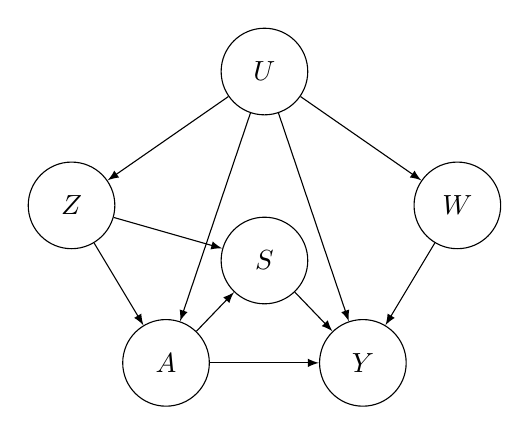
\begin{tikzpicture}[state/.style={circle, draw, minimum size=1.1cm}]
  \def\Ax{0}
  \def\Ay{0}
  \def\offset{2.5}
  \def\Bx{\Ax+5}
  \def\By{\Ay}
  \node[state,shape=circle,draw=black] (Z) at (\Bx-3.7,\Ay+2) {$Z$};
  \node[state,shape=circle,draw=black] (Y) at (\Bx,\By) {$Y$};
  \node[state,shape=circle,draw=black] (A) at (\Bx-2.5,\By) {$A$};
  \node[state,shape=circle,draw=black] (S) at (\Bx-1.25,\By+1.3) {$S$};
  \node[state,shape=circle,draw=black] (U) at (\Bx-1.25,\By+3.7) {$U$};
  \node[state,shape=circle,draw=black] (W) at (\Bx+1.2,\Ay+2) {$W$};

  \draw [-latex] (A) to [bend left=0] (Y);
  \draw [-latex] (A) to [bend left=0] (S);
  \draw [-latex] (Z) to [bend left=0] (S);
  \draw [-latex] (S) to [bend left=0] (Y);
  \draw [-latex] (Z) to [bend left=0] (A);
  \draw [-latex] (W) to [bend left=0] (Y);

  \draw [-latex] (U) to [bend left=0] (A);
  \draw [-latex] (U) to [bend left=0] (Z);
  \draw [-latex] (U) to [bend left=0] (Y);
  \draw [-latex] (U) to [bend left=0] (W);
\end{tikzpicture}
\caption{DAG with latent node $S$.}
\label{fig:figure1}
\end{subfigure}\hfill
\begin{subfigure}[t]{0.48\textwidth}
\centering
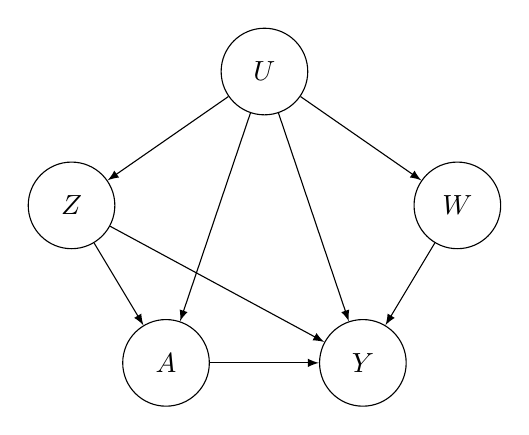
\begin{tikzpicture}[state/.style={circle, draw, minimum size=1.1cm}]
  \def\Ax{0}
  \def\Ay{0}
  \def\offset{2.5}
  \def\Bx{\Ax+5}
  \def\By{\Ay}
  \node[state,shape=circle,draw=black] (Z) at (\Bx-3.7,\Ay+2) {$Z$};
  \node[state,shape=circle,draw=black] (Y) at (\Bx,\By) {$Y$};
  \node[state,shape=circle,draw=black] (A) at (\Bx-2.5,\By) {$A$};
  \node[state,shape=circle,draw=black] (U) at (\Bx-1.25,\By+3.7) {$U$};
  \node[state,shape=circle,draw=black] (W) at (\Bx+1.2,\Ay+2) {$W$};

  \draw [-latex] (A) to [bend left=0] (Y);
  \draw [-latex] (Z) to [bend left=0] (A);
  \draw [-latex] (Z) to [bend left=0] (Y);
  \draw [-latex] (W) to [bend left=0] (Y);

  \draw [-latex] (U) to [bend left=0] (A);
  \draw [-latex] (U) to [bend left=0] (Z);
  \draw [-latex] (U) to [bend left=0] (Y);
  \draw [-latex] (U) to [bend left=0] (W);
\end{tikzpicture}
\caption{Marginal DAG after integrating out $S$.}
\label{fig:figure1.1}
\end{subfigure}

\caption{Extension 2. \subref{fig:figure1}: the DAG that motivates the shape of the working model, with the latent stratum variable $S$ now influenced by $Z$ as well; \subref{fig:figure1.1}: its marginalization over $S$, which augments the classical proximal DAG of Figure \ref{fig:figure1.0} with the edge $Z \to Y$ and on which the underlying model is based. The DAG \subref{fig:figure1} is motivation only and is nowhere assumed.}
\end{figure}
\vspace{-0.5cm}

The same tower-property computation as in Extension~1 turns \eqref{eq: model within stratum} into a stratum-wise linear regression of the observables, $\ex(Y\mid A,S,Z)=\theta_{0,S}^y+\theta_{1,S}^yA+\theta_{2,S}^yZ$; averaging over $S\mid A,Z$, the observables therefore follow the mixture
\begin{align}
    & S \mid A,Z \sim (w_k(A,Z))_{k \in \mathbb{N}} \label{eq: weights distr} \\
    &Y \mid A, Z \sim \sum_{k =1}^{\infty} w_k (A,Z) \,  N(\theta_{0,k}^{y} + \theta_{1,k}^{y} A + \theta_{2,k}^{y} Z, \sigma^2_{y,k}) \\
    & W \mid A,Z \sim N(\theta_{0}^{w} + \theta_{1}^{w} A + \theta_{2}^{w} Z, \sigma^2_{w}) \label{eq: law of W|A,Z 2}
\end{align}
with $(\theta^y_{i,k})_{i\in\{0,1,2\},k\in\mathbb{N}}$, $(\theta^w_i)_{i\in\{0,1,2\}}$ and $(w_k(A,Z))_{k\in\mathbb{N}}$ now treated as free parameters, rather than fixed at the values determined by the betas above, that we fit to a sample $(Z,A,Y,W)$ via the Bayesian nonparametric procedure of Section~\ref{sec: estimation}. 

The following theorem is the analogue of Theorem \ref{thm: extension 1}: part (a) identifies the ATE of the underlying model by an explicit functional of the laws of the observables, and part (b) turns this functional into the closed form computed by the fitted working model. The contrast with Extension 1 lies in the stratum representation required in part (b): a stratum structure on the observables alone no longer suffices, and the representation must now involve the unobserved confounder $U$; unlike in Extension 1, the working model does not automatically supply such a representation, since the mixture \eqref{eq: weights distr}--\eqref{eq: law of W|A,Z 2} is fitted to the observables alone and says nothing, by itself, about $U$. Its existence is therefore a genuine compatibility condition between the underlying model and the stratum structure of the working model.

\begin{theorem}[Extension 2]\label{thm: extension 2}\label{lemma: identify EYa from data}\label{prop: underlying}\label{prop: equivalence ATE}
Suppose $(U,Z,A,Y,W)$ follows the underlying model: the DAG of Figure \ref{fig:figure1.1} (hence the consistency \ref{ass 1} and the conditional independence \ref{ass 2}) and
\begin{enumerate}
\item For some measurable $f_0$ and functions $\alpha_0,\alpha_1$,
\[
\ex(Y\mid A,U,Z)= f_0(A,Z) + \{\alpha_0(A)+\alpha_1(A)Z\}U;
\]
\item $\ex(W\mid A,U,Z)=\beta_0^w+\beta_1^w U$ with $\beta_1^w\neq 0$;
\item $\ex(U\mid A,Z)=\beta_1^u A+\beta_2^u Z$ with $\beta_2^u\neq 0$.
\end{enumerate}
Fix $a \in \mathcal{A}$, let $Q_a$ denote the conditional law of $Z\mid A=a$, and assume moreover:
\begin{enumerate}
\item[(i)] (Orthogonality) $\ex[f_0(a,Z)Z^j\mid A=a]=0$ for $j=0,1,2$;
\item[(ii)] (Invertibility) $G_a=\ex[\phi(Z)\phi(Z)^\top\mid A=a]$ with $\phi(Z)=(1,Z,Z^2)^\top$ is invertible.
\end{enumerate}
Then:
\begin{enumerate}[label=\textup{(\alph*)}]
\item (Identification) $\ex(W\mid A,Z)=\theta_0^w+\theta_1^wA+\theta_2^wZ$ with $\theta_2^w = \beta_1^w\beta_2^u \neq 0$, and the ATE admits the representation
\begin{align}\label{eq: ATE underlying ext2}
\ex \, Y(a)
=
\ex[\ex(Y\mid A=a,Z)]
+
\ex\!\left[
\gamma(a,Z)\,
\{\ex(W\mid A,Z)-\ex(W\mid A=a,Z)\}
\right],
\end{align}
where $\gamma(a,z)$ is identified from the laws of the observables:
\[
\gamma(a,z)=\frac{1}{\theta_2^w}\Big\{ b_1(a)+b_2(a)\Big(z-a\frac{\theta_1^w}{\theta_2^w}\Big)\Big\},
\]
with $(b_0(a),b_1(a),b_2(a))$ the $L_2(Q_a)$-projection coefficients of $\ex(Y\mid A,Z)$ onto the $\mathrm{span}\{1,z,z^2\}$.
\item (Closed form under a stratum representation) Let $(U,Z,A,Y,W,S)$ be any stratum representation of the \emph{full} vector, including the unobserved confounder: a random vector, on some probability space, whose first five coordinates are distributed as $(U,Z,A,Y,W)$ and such that
\begin{align}
        S \independent U \mid A,Z \qquad \text{and} \qquad \ex(Y \mid A,U,S,Z) = \beta_{0,S}^{y} + \beta_{1,S}^{y} A + \beta_{2,S}^{y} U, \label{eq: stratum structure ext2}
\end{align}
for some coefficients $(\beta^y_{i,s})_{i \in \{0,1,2\}, s \in \mathbb{N}}$, and suppose $\mathrm{Var}(U \mid A=a,Z) > 0$ $Q_a$-a.s., i.e.\ the confounder is not a deterministic function of the observed covariates. Then there exist coefficients $(\theta^y_{i,s})_{i \in \{0,1,2\}, s \in \mathbb{N}}$ such that
\begin{align}
        \ex(Y \mid A,S,Z) = \theta_{0,S}^{y} + \theta_{1,S}^{y} A + \theta_{2,S}^{y} Z, \label{eq: 2a.2}
\end{align}
and, for $\boldsymbol{\theta}_{i}(a,Z):=\ex(\theta_{i,S}^{y}\mid A=a,Z),\, i=0,1,2$,
\[
\frac{\boldsymbol{\theta}_2(a,Z)}{\theta_2^w}=\gamma(a,Z) \quad Q_a\text{-a.s.},
\]
so the ATE takes the closed form
\begin{align}\label{eq: rewriting treatment effect}
\ex \, Y(a) &=\ex\,\ex(Y\mid A=a,Z)
+\ex\!\left[\frac{\boldsymbol{\theta}_2(a,Z)}{\theta_2^w}\big(\ex(W\mid A,Z)-\ex(W\mid A=a,Z)\big)\right] \nonumber\\
&= \ex\!\left[\boldsymbol{\theta}_0(a,Z)+\boldsymbol{\theta}_1(a,Z)\,a-\frac{\boldsymbol{\theta}_2(a,Z)}{\theta_2^w}\big(\theta_0^w+\theta_1^w a\big)\right]
+\ex\!\left[\frac{\boldsymbol{\theta}_2(a,Z)}{\theta_2^w}\,W\right].
\end{align}
\end{enumerate}
\end{theorem}

The \hyperlink{proof of thm extension 2}{proof} of Theorem \ref{thm: extension 2} is provided in the Appendix.

\begin{remark}
By the tower property, condition \eqref{eq: stratum structure ext2} combined with $S\independent U\mid A,Z$ implies $\ex[\beta_{2,S}^y\mid A,Z]=\alpha_0(A)+\alpha_1(A)Z$. This represents a genuine constraint for the augmented joint of $(U,Z,A,Y,W,S)$.
\end{remark}

After choosing a prior for $((\theta^y_{i,k} )_{k \in \mathbb{N}, i \in \{0,1,2\} }, (\theta^w_{i} )_{ i \in \{0,1,2\} }, (w_k(A, Z))_{k \in \mathbb{N}} )$, any posterior draw of the parameters of the working model \eqref{eq: weights distr}-\eqref{eq: law of W|A,Z 2} defines a stratum structure on the fitted law of the observables, with $\boldsymbol{\theta}_i(a,Z) = \sum_k w_k(a,Z)\,\theta^y_{i,k}$, and the closed form \eqref{eq: rewriting treatment effect} of Theorem \ref{thm: extension 2}(b) reads
\begin{align*}
\ex \, Y(a) =
\sum_{k\ge 1}\ex\!\left[w_k(a,Z)\left(\theta_{0,k}^{y}+\theta_{1,k}^{y}a-\frac{\theta_{2,k}^{y}}{\theta_2^{w}}(\theta_0^{w}+\theta_1^{w}a)\right)\right] +
\sum_{k\ge 1}\frac{\theta_{2,k}^{y}}{\theta_2^{w}}\ex\!\left[w_k(a,Z)\,W\right],
\numberthis \label{eq: first formula to rewrite Z plugin}
\end{align*}
so the posterior on the parameters induces, through \eqref{eq: first formula to rewrite Z plugin}, a posterior on the ATE. The scope of this procedure is again given by the theorem, with one difference from Extension 1: the fitted mixture provides strata for the observables only, whereas part (b) requires a stratum representation involving the unobserved confounder, as in \eqref{eq: stratum structure ext2}. The quantity estimated by \eqref{eq: first formula to rewrite Z plugin} therefore equals $\ex \, Y(a)$ under every underlying model for which the fitted stratum structure extends to a representation compatible with the confounder. By part (a), consistent estimation of the regressions of the observables still translates into consistent estimation of the ATE. Corollary \ref{corollary: consistency ATE} in Section \ref{sec: estimation} makes this precise for the Bayesian procedure that we propose.

The representation \eqref{eq: ATE underlying ext2} also clarifies the role of the proximal correction in this extended setting: $\ex\, Y(a)$ separates into a baseline outcome regression term, $\ex[\ex(Y\mid A=a,Z)]$, and a proxy-based bias-correction term driven by $\ex(W\mid A,Z)-\ex(W\mid A=a,Z)$. Hence, the departure from standard outcome-regression identification is entirely encoded in the second term, whose weight $\gamma(a,Z)$ is itself identified from observable regressions. This decomposition is useful both conceptually and practically. Conceptually, it shows that allowing the edge $Z \to Y$ does not invalidate proximal identification; rather, it changes the form of the bridge through $\gamma(a,Z)$ while preserving identification from observables. Practically, the theorem gives transparent sufficient conditions for consistency: accurate recovery of $\ex[Y \mid A=a, Z=z]$ and $\ex[W \mid A=a, Z=z]$, together with stable estimation of $(\theta_1^w,\theta_2^w)$ and a non-degenerate denominator $|\theta_2^w|>0$. In particular, weak signal in $\theta_2^w$ is the main source of instability, so inference should be accompanied by diagnostics on the strength of the $Z$-coefficient in the $W$-model.

\begin{remark}[Possible extension]
A natural extension of Proposition \ref{prop: underlying} is to replace the linear interaction in \(Z\), $\{\alpha_0(A)+\alpha_1(A)Z\}U,$ by a richer dictionary interaction
$\big\{\alpha_0(A)+\sum_{k=1}^K \alpha_k(A)\varphi_k(Z)\big\}U$. 

Under the same proximal assumptions on \(W\) and \(U\), together with the analogous orthogonality and invertibility conditions for the enlarged basis
\[
\psi(Z)=(1,\varphi_1(Z),\ldots,\varphi_K(Z),Z,Z\varphi_1(Z),\ldots,Z\varphi_K(Z)),
\]
one expects the same bridge form
\[
\ex\, Y(a)
=
\ex[\ex(Y\mid A=a,Z)]
+
\ex\!\left[\gamma(a,Z)\{\ex(W\mid A,Z)-\ex(W\mid A=a,Z)\}\right],
\]
with \(\gamma(a,Z)\) identified through \(L_2(Q_a)\)-projection coefficients on \(\mathrm{span}\{\psi\}\). In that extension, writing
\[
b(a)=G_a^{-1}\ex[\ex(Y\mid A=a,Z)\psi(Z)\mid A=a],
\]
with components
\[
b(a)=\big(b_0(a),\,b_{\varphi_1}(a),\ldots,b_{\varphi_K}(a),\,b_Z(a),\,b_{Z\varphi_1}(a),\ldots,b_{Z\varphi_K}(a)\big),
\]
the corresponding bridge coefficient is
\[
\gamma(a,z)
=
\frac{1}{\theta_2^w}
\left\{
b_Z(a)
+
\sum_{k=1}^K b_{Z\varphi_k}(a)\varphi_k(z)
-
a\frac{\theta_1^w}{\theta_2^w}
\sum_{k=1}^K b_{\varphi_k}(a)\varphi_k(z)
\right\}.
\]
\end{remark}




\section{Contraction}\label{sec: estimation}


In this section, we present the key theorems that provide sufficient conditions for posterior consistency of the ATE within a class of underlying causal models. We state the results for the second extension of the linear model (DAG~\ref{fig:figure1}). The analogous results for the first extension (DAG~\ref{fig:figure2}) do not follow automatically: in that simpler model the mixture weights $w_k(A)$ depend only on $A$, so the prior has strictly smaller support than the covariate-dependent prior used here. The KL property and the sieve entropy bound (Theorems~\ref{thm: f KL property} and~\ref{thm: consistency tilde{f}}) were established for the covariate-dependent weights \eqref{eq: weights}; extending them to $A$-only weights requires verifying that the true density $f_0(\cdot\mid a,z)$ lies in the support of the restricted prior, which holds when $f_0$ itself depends on $(a,z)$ only through $a$. Under that restriction the proofs carry over verbatim, and we leave the straightforward adaptation to the reader.


\subsection{ \textit{Priors}}

For the law $\mathcal{L}(W \mid A,Z)$ we fit a parametric model normal as follows:
\begin{align*}
    W \mid A,Z \sim N(\theta_{0}^w + \theta_{1}^w A + \theta_{2}^w Z, \sigma^2_{w})      \numberthis \label{eq: law of W|A,Z 3}
\end{align*}
The prior on the weights $\boldsymbol{\theta}^w := (\theta_{0}^w, \theta_{1}^w ,\theta_{2}^w)$ is a normal with mean $\mu_{ \scriptscriptstyle{\boldsymbol{\theta}^w}}$ and diagonal covariance matrix $\Sigma_w$. We put an Inverse Gamma prior on the standard deviation $\sigma_w \sim \mathrm{InvGamma}(\gamma_1, \gamma_2)$.

On the other hand, for the law of the observables $\mathcal{L}(Y \mid A,Z)$ we fit a nonparametric predictor dependent countable mixture of Gaussian linear regressions:
\begin{align*}
     Y \mid A, Z \sim \sum_{k =1}^{\infty} w_k^n (A,Z) \,  N(\theta_{0,k}^y + \theta_{1,k}^y A + \theta_{2,k}^y Z, \sigma^2_{y,k}) \numberthis \label{eq: law of Y|A,Z 3}
\end{align*}
The nonparametric aspect of this prior consists in the construction of the weights $(a,z) \mapsto w_k^n (a,z)$ for all $k,n \in \mathbb{N}$.
For $k \in \mathbb{N}$ consider three independent discrete-time Gaussian sequences $\{ \eta_{i,m}^k \}_{m=1}^{\infty}$, $i=0,1,2$, supported on $\mathbb{N}$ such that, for integer $l\geq 0$: 
\begin{align}
    \ex \eta^k_{i,m} = \mu_{i,m}^k \quad \text{and} \quad \operatorname{Cov}(\eta_{i,m}^k, \eta_{i,m+l}^k) = {}_{k}{\sigma}^2_{i,m} \delta_m(m+l), \quad \quad i=0,1,2, \, \, \forall \, k \in \mathbb{N}.
\end{align}
Thus $\forall \, m, k \in \mathbb{N}$, $\boldsymbol{\mu}_m^k = (\mu_{0,m}^k, \mu_{1,m}^k, \mu_{2,m}^k)$ and $\Sigma_m^k = \operatorname{diag}({}_{k}{\sigma}^2_{0,m}, {}_{k}{\sigma}^2_{1,m}, {}_{k}{\sigma}^2_{2,m})$, $\boldsymbol{\eta}_m^k \sim N(\boldsymbol{\mu}_m^k, \Sigma_m^k) $ and $\boldsymbol{\eta}_m^k \independent \boldsymbol{\eta}_l^k$ for $l \neq m$. 

Now for realizations $A=a$, $Z=z$, define $\boldsymbol{x}= (a,z)$. Then for integers $N_n \rightarrow \infty$ as $n\rightarrow \infty$, define, for every fixed $n\in \mathbb{N}$ partitions $\cup_{m=1}^{N_n} T_{m,n}$ of the domain $\mathcal{X}= \mathcal{A} \times \mathcal{Z}$ of the covariate space:
\begin{align}
    &\alpha_k^n(\boldsymbol{x}) = \sum_{m=1}^{N_n} (\eta_{0,m}^k + \eta_{1,m}^k a + \eta_{2,m}^k z) \ind_{(a,z) \in T_{m,n}} \numberthis \label{eq: alpha} \\
    &w_k^n(\boldsymbol{x}) = \Phi(\alpha_k^n(\boldsymbol{x})) \prod_{l<k} \left\{ 1- \Phi(\alpha_l^n(\boldsymbol{x}))\right\} \numberthis \label{eq: weights}
\end{align}
where $\Phi (\cdot)$ denotes the cumulative distribution function for the standard normal distribution.  We thus conclude that the prior is given by the dependent probit-stick breaking mixtures of normals, for $\bar{\boldsymbol{x}} = (1,a,z)$ and for a base measure $G_0$:
\begin{align*}
    &G^n_{\boldsymbol{x}} = \sum_{k=1}^{\infty} w_k^n (\boldsymbol{x}) \delta_{(\boldsymbol{\theta}^y,\sigma_y)}, \quad \quad (\boldsymbol{\theta}^y,\sigma_y) \sim G_0 \numberthis \label{eq: almost end definition prior}\\
    &f(y \mid \boldsymbol{x}) = \int \frac{1}{\sigma_y} \phi \left( \frac{y- \bar{\boldsymbol{x}}^{\prime} \boldsymbol{\theta}^y}{\sigma_y}\right) \, d G^n_{{\boldsymbol{x}}}(\boldsymbol{\theta}^y,\sigma_y) \numberthis \label{eq: end definition prior}.
\end{align*}
Note that $w^n_k(\boldsymbol{x}) \geq 0$ are random functions of $\boldsymbol{x}$ such that $\sum_{k=1}^{\infty} w^n_k(\boldsymbol{x})=1$ a.s. for each fixed $\boldsymbol{x} \in \mathcal{X}$ and $G_0=G_{0, \boldsymbol{\theta}^y} \times G_{0, \sigma_y}$ is a probability distribution on $\mathbb{R}^3 \times \mathbb{R}^{+}$where $G_{0, \boldsymbol{\theta}^y}$ and $G_{0, \sigma_y}$ are probability distributions on $\mathbb{R}^3$ and $\mathbb{R}^{+}$ respectively. We additionally assume that the prior satisfies the following two properties, where we denote the supremum norm on the covariate space by $\| \cdot \|$ and the variance by $\mathbb{V}$: $0 < \min_{ 1 \leq k \leq m_n}\|\mathbb{V}(\alpha_k^n) \| \leq \max_{ 1 \leq k \leq m_n}\|\mathbb{V}(\alpha_k^n) \| <\infty, \quad \forall \, n \in \mathbb{N}.$




\subsection{\textit{Results}}

Assume the $Y_i $ is observed independently given the covariates $ (A_i,Z_i)$, $i=1,2,\ldots$ which are drawn independently from a probability distribution $Q$ on $\mathcal{X}$ which admits density $q$ with respect to the Lebesgue measure and which is known. Similarly the $W_i$ is observed independently given the covariates $ (A_i,Z_i)$, $i=1,2,\ldots$. Denote the observed data of size $n$ by $\mathcal{D}^{(n)} = (Y^{(n)}, W^{(n)}, A^{(n)}, Z^{(n)})$, where $x^{(n)} = (x_1,\ldots,x_n)$. We denote by $p_0$ the joint density of $Y,W,A,Z$ relative to the probability measure $P_0$. Given the prior $\Pi$ we denote a version of the posterior by  $\Pi_n\left(\cdot \mid \mathcal{D}^{(n)} \right)$.

We assume $q$ is known, but it could be estimated separately from the data. Note that our model in Section \ref{sec: mixture of normals} does not impose any restriction on $q$. There are several well known nonparametric estimation methods in the literature that under mild restrictions give consistency in density estimation (e.g.\ Dirichlet Process Mixtures or exponential transforms of Gaussian Process, see \cite{4}). 

Now we present the main result of this section, which confirms consistency of the ATE when using the above constructed priors. Most of the proofs of this section are based on existing work done in \cite{202} and \cite{121}.

\begin{corollary}\label{corollary: consistency ATE}
    Consider any underlying causal model that satisfies the assumptions of Proposition \ref{prop: underlying} and assume the joint law $Q$ of $Z,A$ as well as the conditional law $Q_a$ of $Z\mid A=a$ with density $z \mapsto q(z \mid a)$ for any fixed $a \in \mathcal{A}$ are known. Consider the prior defined in \eqref{eq: law of W|A,Z 3}-\eqref{eq: end definition prior}. Suppose furthermore that the assumptions of Theorem \ref{thm: consistency tilde{f}} and Proposition \ref{prop: consistency para} are satisfied, and that:
    \begin{itemize}
        \item[A.] There exists a constant $C < \infty$ such that
        \[
        \Pi_n\!\left(\sup_{(a,z)\in\mathcal{X}}\int y^2 f(y\mid a,z)\,dy \leq C \,\Big|\, \mathcal{D}^{(n)}\right) \to 1, \quad P^{(n)}_0\text{-a.s.}
        \]
    \end{itemize}
    Then for every fixed $a \in \mathcal{A}$:
    \begin{align}
        \Pi_n ( |\ex_0 Y(a) - \ex \, Y(a)| > \varepsilon \mid \mathcal{D}^{(n)}) \rightarrow 0, \quad \quad P^{(n)}_0-\text{a.s.}
    \end{align}
\end{corollary}
\begin{remark}
Assumption~A is a mild posterior regularity condition. It is implied, for instance, if the sieve $\mathcal{F}_n^a$ in the proof of Theorem~\ref{thm: consistency tilde{f}} is further restricted to have component parameters $\|\boldsymbol{\theta}_k^y\| \leq R$ and $\sigma_{y,k} \leq R$ for a fixed constant $R < \infty$ independent of $n$, since in that case $\int y^2 f(y\mid a,z)dy \leq R^2(1+|a|+|z|)^2 + R^2 \leq 4R^2(1+C_{\mathcal{X}})^2$ uniformly over $(a,z)\in\mathcal{X}$ and over the truncated sieve. Moreover, under the underlying model the true second moment $\int y^2 f_0(y\mid a,z)dy = \mathrm{Var}(Y\mid A=a,Z=z) + m_Y^0(a,z)^2$ is bounded uniformly over compact $\mathcal{X}$ by the assumptions of Proposition~\ref{prop: underlying}, so the true density automatically satisfies the same bound.
\end{remark}
The \hyperlink{proof of corollary}{proof} of this corollary is a consequence of Theorem \ref{thm: consistency tilde{f}}, Proposition \ref{prop: consistency para} (provided below) and the triangle inequality and it is provided in Appendix B. We now outline the main results involved in the proofs that lead to the conclusion of Corollary \ref{corollary: consistency ATE}. 

Because we are concerned with consistency of the distributions of $Y \mid A,Z \sim f_0( \cdot \mid A,Z)$ and of $ W \mid A,Z \sim g_0( \cdot \mid A,Z)$, we have that the marginals of interest are:
\begin{align*}
    &h^y_0(y,a,z) = f_0(y \mid a,z) q(a,z), \quad \quad h^w_0(w,a,z) = g_0(w \mid a,z) q(a,z).
\end{align*}
Recall $\boldsymbol{x} = (a,z)$. For $f_0 \in \mathcal{F}_d$ such that $h^y_0(\boldsymbol{x}, y)=q(\boldsymbol{x}) f_0(y \mid \boldsymbol{x})$ is the true joint data-generating density, where $\mathcal{F}_d$ is the space of conditional densities which are continuous in its arguments (see Def. \ref{def: F_d}), we define an $\varepsilon$-sized KL neighborhood around $f_0$. 
For $\operatorname{KL}\left(h^y_0, h^y\right)=\int h^y_0 \log \left(h^y_0 / h^y \right)$: 
\begin{align}
  K_\varepsilon\left(f_0\right)=\left\{f: f \in \mathcal{F}_d, \operatorname{KL}\left(h^y_0, h^y \right)<\varepsilon, h^y(\boldsymbol{x}, y)=q(\boldsymbol{x}) f(y \mid \boldsymbol{x}), \, \, \forall \, y \in \mathcal{Y}, \boldsymbol{x} \in \mathcal{X}\right\}  
\end{align}
Then, $\Pi_n$ is said to have KL property at $f_0 \in \mathcal{F}_d$, denoted $f_0 \in \operatorname{KL}\left(\Pi_n\right)$, if, $\forall \, \varepsilon >0$: 
$$\liminf_{n \rightarrow \infty} \Pi_n\left\{K_\varepsilon\left(f_0\right)\right\}>0.$$
\begin{remark}
    Note that $f_0 \in \operatorname{KL}\left(\Pi_n\right)$ implies $\forall \, \varepsilon > 0$, as $n \rightarrow \infty$ :
    \begin{align}\label{eq: weak convergence}
    \Pi_n\left(f \, : \, d_w\left(f, f_0\right)>\varepsilon \mid \mathcal{D}^{(n)}\right) \rightarrow 0, \quad \quad \text{in} \, P^{(n)}_0-\text{probability}.
    \end{align}
    $d_w$ is the metric relative to the weak neighborhoods, whose sub-base is defined in \eqref{eq: weak f neighborhoods}.
\end{remark}

\begin{theorem}\label{thm: f KL property}
Consider the prior defined in \eqref{eq: law of Y|A,Z 3}-\eqref{eq: end definition prior}. Assume $\mathcal{X}$ is a compact subset of $\mathbb{R}^3$. If:
\begin{itemize}
    \item[A0.] the base measure $G_0$ is absolutely continuous with respect to $\lambda\left(\mathbb{R}^3 \times \mathbb{R}^{+}\right)$.
    \item[A1.] $f_0$ is nowhere zero and bounded by $M<\infty$.
    \item[A2.] $\left|\int_{\mathcal{X}} \int_{\mathcal{Y}} f_0(y \mid \boldsymbol{x}) \log f_0(y \mid \boldsymbol{x}) \, d y \, q(\boldsymbol{x}) \, d \boldsymbol{x} \right|<\infty$.
    \item[A3.] $\left|\int_{\mathcal{X}} \int_{\mathcal{Y}} f_0(y \mid \boldsymbol{x}) \log \frac{f_0(y \mid \boldsymbol{x})}{\psi_{\boldsymbol{x}}(y)} \, d y \, q(\boldsymbol{x}) \, d \boldsymbol{x}\right|<\infty$, where $\psi_{\boldsymbol{x}}(y)=\inf_{t \in[y-1, y+1]} f_0(t \mid \boldsymbol{x})$.
    \item[A4.] $\exists \, \eta>0$ such that $\int_{\mathcal{X}} \int_{\mathcal{Y}} |y|^{2(1+\eta)} f_0(y \mid \boldsymbol{x}) \, d y \, q(\boldsymbol{x}) \, d \boldsymbol{x}<\infty$.
    \item[A5.] $(\boldsymbol{x}, y) \mapsto f_0(y \mid \boldsymbol{x})$ is jointly continuous.
\end{itemize}
Then $f_0 \in \operatorname{KL}\left(\Pi_n\right)$.
\end{theorem}

The \hyperlink{proof of thm KL property}{proof} of Theorem \ref{thm: f KL property} is given in Appendix B. Because we adopted a parametric model for the law $\mathcal{L}(W \mid A,Z)$ consistency of the functional $\ex[W \mid Z]$ and $\ex [W \mid A=a, Z]$ in $\mathbb{L}_1$ is easily granted. The \hyperlink{proof of prop para}{proof} of this proposition, provided in Appendix B, is a straightforward application of the standard theory of consistency for parametric models. 

\begin{proposition}\label{prop: consistency para}
    Under the assumption that the underlying law of $W \mid A,Z$ is as in Proposition \ref{prop: underlying}, that the density $(a,z) \mapsto q (z \mid a)$ is bounded, that the covariate space $\mathcal{W}$ is a bounded subset of $\mathbb{R}$, and using the prior \eqref{eq: law of W|A,Z 3}, for fixed $a \in \mathcal{A}$ and $\forall \, \varepsilon >0$, as $n \rightarrow \infty$:
    \begin{align*}
        &\Pi ( \, \ex_0 | 
\ex_0 (W\mid A=a,Z)- \ex(W\mid A=a,Z) | > \varepsilon \mid \mathcal{D}^{(n)}) \rightarrow 0, \quad \quad P^{(n)}_0-\text{a.s.} \\
        &\Pi ( \, \ex_0 | 
\ex_0 (W\mid A,Z)- \ex(W\mid A,Z) | > \varepsilon \mid \mathcal{D}^{(n)}) \rightarrow 0, \quad \quad \quad \quad \quad \, \, \, \, P^{(n)}_0-\text{a.s.}
    \end{align*}
    where $\ex_0 | \ex_0 (W\mid A,Z)- \ex(W\mid A,Z) | = \iint |\int w (g_0(w\mid a,z)- g(w\mid a,z)) \, dw | \, q(a, z) \, d a \, d z$ and $\ex_0 | \ex_0 (W\mid A=a,Z)- \ex(W\mid A=a,Z) | = \iint |\int w (g_0(w\mid a,z)- g(w\mid a,z)) \, dw | \, q(z \mid a) \, d z$.
\end{proposition}

We now prove consistency in $\mathbb{L}_1$ integrated with respect to the density $q(z \mid a)$ (see the metric defined by \eqref{eq: a-L1 integrated neighborhood f} in Appendix A). For fixed $a \in \mathcal{A}$ let $(a,z) \mapsto q(z \mid a)$ be the density of the underlying probability measure associated to the law of $Z \mid A$. Then we denote the joints:
\begin{align*}
    &f^a_0(y,z\mid a) = f_0(y \mid a,z) \, q(z \mid a) \numberthis \label{eq: f^a_0}
\end{align*}
Note that the metric of interest (c.f.\ \eqref{eq: a-L1 integrated neighborhood f}) can be conveniently rewritten as follows using Fubini's theorem and the nonnegativity of $z \mapsto q (z \mid a)$ for fixed $a \in \mathcal{A}$: 
\begin{align*}
    \int \left\|f(\cdot \mid a,z) - f_0(\cdot \mid a,z)\right\|_{1} q(z \mid a) \, d z &= \int \int |f(y \mid a,z) - f_0(y \mid a,z)| \, q(z \mid a) \, d z \, dy \\
    &= \| f^a_0 - f^a \|_1.
\end{align*}
\begin{theorem}\label{thm: consistency tilde{f}}
    Fix $a \in \mathcal{A}$. Consider the prior defined in \eqref{eq: law of Y|A,Z 3}-\eqref{eq: end definition prior}. Let the assumptions of Theorem \ref{thm: f KL property} hold true. Assume $\mathcal{X}$ is a compact subset of $\mathbb{R}^3$ and that, for fixed $a \in \mathcal{A}$, the assumptions of Theorem \ref{thm: f KL property} are satisfied with respect to the density $z \mapsto q(z \mid a)$. Moreover if:
    \begin{itemize}
        \item[B0.] the base measure $G_0$ satisfies $G_0 \left(([-a_n,a_n]^3)^c \times [l_n,h_n]^c\right) \leq m_n^{-1} e^{-m_n \log{m_n}}$, where $a_n = \sqrt{n}$, $h_n = \sqrt{n}$, $l_n = 1/\sqrt{n}$, $m_n = n/\log{n}$.
        \item[B1.] for any fixed $a \in \mathcal{A}$, $(z,y) \mapsto f_0(y \mid a,z)$ is jointly continuous.
    \end{itemize}
    Then $\forall \, \varepsilon > 0$, as $n \rightarrow \infty$ :
    $$
    \Pi_n\left( f \, : \, \| f^a- f^a_0\|_1>\varepsilon \mid \mathcal{D}^{(n)}\right) \rightarrow 0, \quad \quad P^{(n)}_0-\text{a.s.}
    $$
\end{theorem}
The \hyperlink{proof of thm consistency f tilde}{proof} of Theorem \ref{thm: consistency tilde{f}} is provided in Appendix B. This result is the last fundamental piece that leads to consistency of the ATE, since it gives consistency in $\mathbb{L}_1$ metric for the density of $Y \mid A, Z$ when modelled with the Bayesian nonparametric procedure we proposed.

\section{Conclusion}
  
In this chapter, we introduced a more versatile approach to causal inference when unmeasured confounding is present. By building upon the classical linear model in the setting of proximal inference and transitioning to mixtures of linear models, we created a more flexible framework for modeling the distribution of outcomes given the covariates. We proved that in this framework the average treatment effect remains identifiable and, by deriving it, we obtained a closed-form expression for the bridge function. This extension improves on the limitations of simpler linear models, which often fail to capture the intricacies of real-world data.

Additionally, we presented a Bayesian nonparametric estimation method that employs a probit stick-breaking process with mixing weights that depend on the covariates. Our findings indicate that this method yields consistency across various causal models. One significant benefit of our approach is its guarantee of the bridge function's existence, which simplifies the estimation process within this framework. Although our method enhances flexibility, it still relies on assumptions regarding the simpler linear model for the distribution of $W$ given the covariates. Future studies could explore relaxing these assumptions to further extend the model's applicability. Nevertheless, our work represents a substantial advancement in proximal inference, offering a practical solution for estimating the average causal effect in presence of unmeasured confounding.




\section{Appendix}\label{sec: appendix chapter5}

\subsection{Definitions of function spaces and topologies used in proofs}

First we define all the relevant function spaces for our consistency study.
\begin{definition}\label{def: F_d}
Let $\mathcal{X}= \mathcal{A} \times \mathcal{Z}$ be the covariate space which is a compact subset of $\mathbb{R}^2$ and $\mathcal{Y} = \mathbb{R}$ be the response space. Let:
\begin{align*}
    \mathcal{F}_d=&\bigg\{f: \mathcal{X} \times \mathcal{Y} \rightarrow (0, \infty), \int f(y \mid \boldsymbol{x}) \, d y = 1, \, \forall \, \boldsymbol{x} \in \mathcal{X} \, \text{and the map from} \, \\
    &\quad \boldsymbol{x} \mapsto \mathbb{L}_1(\lambda, \mathcal{Y}), \, \boldsymbol{x} \mapsto f(\cdot \mid \boldsymbol{x}) \, \,  \text{is continuous} \bigg\}.
\end{align*}
Similarly, we define the space $\mathcal{G}_d$ for the conditional densities $g : \mathcal{X} \times \mathcal{W} \rightarrow (0, \infty)$.
\end{definition}

\begin{definition}\label{def: set G*}
Define collection of conditional probability measures on $(\mathbb{R}^3 \times \mathbb{R}^+, \mathcal{B} (\mathbb{R}^3 \times \mathbb{R}^{+} ) )$ denoted by $\mathscr{G}_x^{*}$ such that $ \forall \, B \in \mathcal{B}(\mathbb{R}^3 \times \mathbb{R}^{+})$, 
\begin{itemize}
\item $\boldsymbol{x} \mapsto F_{\boldsymbol{x}}(B)$ is continuous,
\item  for any sequence of sets $A_n \subset \mathbb{R}^3 \times \mathbb{R}^+ \downarrow \emptyset$, $\sup_{\boldsymbol{x} \in \mathcal{X}} F_{\boldsymbol{x}}(A_n) \downarrow 0$.
\end{itemize}
\end{definition}

We now define all the relevant neighborhoods for our consistency study. For the mixing measures $G_{\boldsymbol{x}} \in \mathscr{G}_x^{*}$ we consider two types of neighborhoods. 

\begin{definition}
For a bounded continuous function $g: \mathbb{R}^3 \times \mathbb{R}^{+} \times \mathcal{X} \rightarrow \mathbb{R}$ and $\varepsilon>0$, a sub-base of the weak neighborhood of a conditional probability measure $\left\{F_{\boldsymbol{x}}, \boldsymbol{x} \in \mathcal{X}\right\}$ is defined as
\begin{align}\label{eq: weak neighborhoods}
    S^w_{\varepsilon}(F_{\boldsymbol{x}},q) := \left\{ \left\{G_{\boldsymbol{x}}: \boldsymbol{x} \in X\right\}: \left| \int_{\mathcal{X} \times \mathbb{R}^3 \times \mathbb{R}^+}   g(\boldsymbol{\theta}, \sigma, \boldsymbol{x}) d\left(G_{\boldsymbol{x}}(\boldsymbol{\theta}, \sigma)-F_{\boldsymbol{x}}(\boldsymbol{\theta}, \sigma)\right)  q(\boldsymbol{x}) \, d \boldsymbol{x} \right| <\varepsilon \right\}.
\end{align}
\end{definition}


A conditional probability measure $\left\{G_{\boldsymbol{x}}, \boldsymbol{x} \in \mathcal{X}\right\}$ lies in the weak support of $\Pi_n$ if it assigns positive probability to every basic neighborhood generated by the sub-base of the type \eqref{eq: weak neighborhoods}. 

\begin{definition}
A weak $\sup$-neighborhood of a $F_{\boldsymbol{x}} \in \mathscr{G}_x^{*}$ is defined, for $\varepsilon>0$, by:
\begin{align}\label{eq: weak sup integrated neighborhoods}
    S^{\scriptscriptstyle{1}}_{\varepsilon}(F_{\boldsymbol{x}},q) := \left\{\left\{G_{\boldsymbol{x}}: \boldsymbol{x} \in X\right\}:\sup_{\boldsymbol{x} \in \mathcal{X}} \left| \int_{\mathbb{R}^3 \times \mathbb{R}^+}  g(\boldsymbol{\theta}, \sigma) d\left(G_{\boldsymbol{x}}(\boldsymbol{\theta}, \sigma)-F_{\boldsymbol{x}}(\boldsymbol{\theta}, \sigma)\right) \right| <\varepsilon\right\}
\end{align}
$g$ bounded continuous function.
    
\end{definition}

We introduce the weak and \(q\)-integrated neighborhoods for a set of conditional densities \(\{f_0(\cdot \mid \boldsymbol{x}), \boldsymbol{x} \in \mathcal{X}\}\) as follows. 
\begin{definition}
A sub-basis for a weak neighborhood for a set of conditional densities \(\{f_0(\cdot \mid \boldsymbol{x}), \boldsymbol{x} \in \mathcal{X}\}\) is given, for $\varepsilon > 0$, by
\begin{align}\label{eq: weak f neighborhoods}
W_{\varepsilon, k}(f_0) = \left\{f: f \in \mathcal{F}_d, \left|\int_{\mathcal{X} \times \mathcal{Y}} k h^y - \int_{\mathcal{X} \times \mathcal{Y}} k h^y_0\right| < \varepsilon \right\},
\end{align}
where \(k: \mathcal{X} \times \mathcal{Y} \to \mathbb{R}\) is a bounded, continuous function and $h^y(y,\boldsymbol{x}) = f(y \mid \boldsymbol{x}) q(\boldsymbol{x})$. We define the same types of neighborhoods also for $g \in \mathcal{G}_d$.
\end{definition}
A weak neighborhood basis is constructed from finite intersections of sets of the form \eqref{eq: weak f neighborhoods}. 
\begin{definition}
The \(q\)-integrated \(\mathbb{L}_1\) neighborhood is given, for $\varepsilon > 0$, by
\begin{align}\label{eq: L1 integrated neighborhood f}
W_\varepsilon(f_0; q) = \left\{f: f \in \mathcal{F}_d, \int \left\|f(\cdot \mid \boldsymbol{x}) - f_0(\cdot \mid \boldsymbol{x})\right\|_{1} q(\boldsymbol{x}) \, d\boldsymbol{x} < \varepsilon \right\}.
\end{align}
Also in this case we define the same types of neighborhoods for $g \in \mathcal{G}_d$.    
\end{definition}
In the topology defined by \eqref{eq: L1 integrated neighborhood f}, the space \(\mathcal{F}_d\) is regarded as a closed subset of \(\mathbb{L}_1(\lambda \times q, \mathcal{Y} \times \operatorname{supp}(q))\), a complete and separable metric space. As a result, measurability concerns do not emerge under these topologies. It is clear that to obtain consistency for the ATE we need to define new neighborhoods for fixed $a \in \mathcal{A}$.
\begin{definition}
    For any fixed $a \in \mathcal{A}$, the \(q^a\)-integrated \(\mathbb{L}_1\) neighborhood is given, for $\varepsilon > 0$, by
    \begin{align}\label{eq: a-L1 integrated neighborhood f}
    W^a_\varepsilon(f_0; q) = \left\{f: f \in \mathcal{F}_d, \int \left\|f(\cdot \mid a,z) - f_0(\cdot \mid a,z)\right\|_{1} q(z \mid a) \, d z < \varepsilon \right\}.
\end{align}    
Similarly, we define the same neighborhoods for $g \in \mathcal{G}_d$.
\end{definition}
\subsection{Proofs}



\begin{proof}[\hypertarget{proof of thm extension 2}{\textbf{Proof of Theorem}} \ref{thm: extension 2}]
\emph{Part (a).} Write $m_Y(a,z)=\ex(Y\mid A=a,Z=z)$ and $m_W(a,z)=\ex(W\mid A=a,Z=z)$.
By iterated expectation and Assumption~3,
\begin{align*}
\ex(Y\mid A,Z)
&=\ex\{\ex(Y\mid A,U,Z)\mid A,Z\}\\
&= f_0(A,Z)+\{\alpha_0(A)+\alpha_1(A)Z\}\ex(U\mid A,Z)\\
&= f_0(A,Z)+\{\alpha_0(A)+\alpha_1(A)Z\}\{\beta_1^u A+\beta_2^u Z\}.
\end{align*}
Fix $a$ and set $c_0(a)=\beta_1^u a$. Then
\begin{align}
m_Y(a,z)= f_0(a,z) + b_0(a)+b_1(a)z+b_2(a)z^2,
\label{eq:poly-decomp-beta0u0}
\end{align}
with
\begin{align}
b_0(a)=\alpha_0(a)c_0(a),\qquad
b_1(a)=\alpha_0(a)\beta_2^u+\alpha_1(a)c_0(a),\qquad
b_2(a)=\alpha_1(a)\beta_2^u.
\label{eq:b-coefs-beta0u0}
\end{align}

Consider $L_2(Q_a)$ with inner product
$\langle r,s\rangle_a=\ex[r(Z)s(Z)\mid A=a]$.
Let $\mathcal S_a=\mathrm{span}\{1,Z,Z^2\}$ and $\phi(Z)=(1,Z,Z^2)^\top$.
By (i), $f_0(a,\cdot)\perp\mathcal S_a$, hence the polynomial term
$p_a(Z)=b_0(a)+b_1(a)Z+b_2(a)Z^2$ is the $L_2(Q_a)$-projection of $m_Y(a,\cdot)$ onto $\mathcal S_a$.
By (ii), the projection coefficients are uniquely identified via the normal equations,
\[
(b_0(a),b_1(a),b_2(a))^\top
=
G_a^{-1}\ex[m_Y(a,Z)\phi(Z)\mid A=a],
\qquad
G_a=\ex[\phi(Z)\phi(Z)^\top\mid A=a].
\]

Define $g_2(a,z):=\beta_2^u\{\alpha_0(a)+\alpha_1(a)z\}$. Using \eqref{eq:b-coefs-beta0u0}, $\beta_2^u\alpha_1(a)=b_2(a)$ and, since $c_0(a)=\beta_1^u a$,
\[
b_1(a)=\beta_2^u\alpha_0(a)+\alpha_1(a)c_0(a)
\quad\Rightarrow\quad
\beta_2^u\alpha_0(a)=b_1(a)-\alpha_1(a)c_0(a)
=b_1(a)-\frac{b_2(a)}{\beta_2^u}\beta_1^u a.
\]
Therefore
\begin{align}
g_2(a,z)
=
b_1(a)+b_2(a)\Big(z-a\frac{\beta_1^u}{\beta_2^u}\Big).
\label{eq:g2-b-form}
\end{align}

Next, by iterated expectation and Assumption~2,
\begin{align*}
\ex(W\mid A,Z)
&=\beta_0^w+\beta_1^w\ex(U\mid A,Z)
=\beta_0^w+\beta_1^w(\beta_1^u A+\beta_2^u Z)
=:\theta_0^w+\theta_1^wA+\theta_2^w Z,
\end{align*}
where $\theta_1^w=\beta_1^w\beta_1^u$ and $\theta_2^w=\beta_1^w\beta_2^u\neq 0$.
Hence
\begin{align}
\frac{\beta_1^u}{\beta_2^u}=\frac{\theta_1^w}{\theta_2^w}.
\label{eq:ratio-ident}
\end{align}
Combining \eqref{eq:g2-b-form}--\eqref{eq:ratio-ident} yields the identified form
\begin{align}
\frac{g_2(a,z)}{\theta_2^w}
=
\frac{1}{\theta_2^w}\Big\{ b_1(a)+b_2(a)\Big(z-a\frac{\theta_1^w}{\theta_2^w}\Big)\Big\}
=: \gamma(a,z).
\label{eq:gamma-az-form}
\end{align}

We now derive the ATE representation. Using the consistency \ref{ass 1} and the conditional independence \ref{ass 2},
\begin{align*}
\ex\{Y(a)\}
&=\ex\big[\ex\{Y\mid A=a,U,Z\}\big]
=\ex\big[f_0(a,Z)+\{\alpha_0(a)+\alpha_1(a)Z\}U\big].
\end{align*}
Also,
\[
\ex[\ex(Y\mid A=a,Z)]
=\ex\big[f_0(a,Z)+\{\alpha_0(a)+\alpha_1(a)Z\}\ex(U\mid A=a,Z)\big].
\]
Subtracting gives
\[
\ex\{Y(a)\}
=
\ex[\ex(Y\mid A=a,Z)]
+
\ex\!\left[\{\alpha_0(a)+\alpha_1(a)Z\}\{\ex(U\mid A,Z)-\ex(U\mid A=a,Z)\}\right].
\]
Since $\ex(W\mid A,Z)=\beta_0^w+\beta_1^w\ex(U\mid A,Z)$, we have
\begin{align*}
\ex(U\mid A,Z)-\ex(U\mid A=a,Z)
&=
\frac{1}{\beta_1^w}\{\ex(W\mid A,Z)-\ex(W\mid A=a,Z)\} \\
&=
\frac{\beta_2^u}{\theta_2^w}\{\ex(W\mid A,Z)-\ex(W\mid A=a,Z)\}.
\end{align*}
Substitute and recall $g_2(a,Z)=\beta_2^u\{\alpha_0(a)+\alpha_1(a)Z\}$ to obtain
\[
\ex [Y(a)]
=
\ex[\ex(Y\mid A=a,Z)]
+
\ex\!\left[
\frac{g_2(a,Z)}{\theta_2^w}
\{\ex(W\mid A,Z)-\ex(W\mid A=a,Z)\}
\right].
\]
Finally, replace $g_2/\theta_2^w$ by $\gamma(a,Z)$ from \eqref{eq:gamma-az-form}, yielding \eqref{eq: ATE underlying ext2}.

\emph{Part (b).} Since a stratum representation preserves the joint law of $(U,Z,A,Y,W)$, all conditional expectations below may be computed on the space carrying it, where $S$ is available. First, by \eqref{eq: stratum structure ext2} and Assumption~3 of the theorem,
\begin{align*}
 \ex(Y \mid A, Z, S)&=\ex(\ex(Y \mid A, U, Z, S) \mid A, Z, S) = \ex\left(\beta_{0,S}^y+\beta_{1,S}^y A+\beta_{2,S}^y U \mid A, Z, S\right) \\
&=\beta_{0,S}^y+\beta_{1,S}^y A+\beta_{2,S}^y \ex(U \mid A, Z) =\beta_{0,S}^y+\left(\beta_{1,S}^y+\beta_{2, S}^y \beta_1^u\right) A+\beta_{2,S}^y \beta_2^u Z,
\end{align*}
where the third equality uses $S \independent U \mid A,Z$. This is \eqref{eq: 2a.2} with
\begin{align}\label{eq: thetas and betas}
    \left\{\begin{array}{l}
\theta_{0,S}^{y}=\beta_{0,S}^y \\
\theta_{1,S}^{y}=\beta_{1,S}^y+\beta_{2,S}^y \beta_1^u \\
\theta_{2,S}^{y}=\beta_{2,S}^y \cdot \beta_2^u
\end{array}\right.
\end{align}

Next we show that marginalising out $S$ recovers the underlying specification. By \eqref{eq: stratum structure ext2}, i.e.\ the stratum-wise outcome regression together with $S \independent U \mid A,Z$,
\begin{align*}
\ex(Y\mid A,U,Z)
&=\ex\!\big(\ex(Y\mid A,U,S,Z)\mid A,U,Z\big) \\
&=\ex(\beta_{0,S}^{y}\mid A,Z)+\ex(\beta_{1,S}^{y}\mid A,Z)\,A+\ex(\beta_{2,S}^{y}\mid A,Z)\,U,
\end{align*}
while Assumption~1 of the theorem gives $\ex(Y\mid A,U,Z)=f_0(A,Z)+\{\alpha_0(A)+\alpha_1(A)Z\}U$. These are two affine representations of the same regression as a function of $U$: their difference, an affine function of $U$, vanishes on the support of $U \mid A=a,Z=z$, which, for $Q_a$-almost every $z$, contains at least two points because $\mathrm{Var}(U\mid A=a,Z=z)>0$; so both its coefficients are zero (the exact analogue of the argument in the proof of Theorem~\ref{thm: extension 1}(b), with $U$ in place of $Z$). Hence
\begin{equation}\label{eq: enrichment condition}
\ex\!\left(\beta_{2,S}^{y}\mid A=a,Z\right)=\alpha_0(a)+\alpha_1(a)Z,\quad Q_a\text{-a.s.}
\end{equation}
Averaging \eqref{eq: thetas and betas} over $S\mid A=a,Z$ and using \eqref{eq: enrichment condition}:
\[
\boldsymbol{\theta}_2(a,Z)
=\ex\!\left(\theta_{2,S}^y\mid A=a,Z\right)
=\beta_2^u\,\ex\!\left(\beta_{2,S}^y\mid A=a,Z\right)
=\beta_2^u\{\alpha_0(a)+\alpha_1(a)Z\}.
\]
From equations \eqref{eq:b-coefs-beta0u0}--\eqref{eq:gamma-az-form} in the proof of part (a), with $\theta_2^w=\beta_1^w\beta_2^u\neq 0$:
\[
\gamma(a,Z)
=\frac{1}{\theta_2^w}\bigl\{b_1(a)+b_2(a)\bigl(Z-a\tfrac{\theta_1^w}{\theta_2^w}\bigr)\bigr\}
=\frac{\alpha_0(a)+\alpha_1(a)Z}{\beta_1^w},
\]
so that
\[
\frac{\boldsymbol{\theta}_2(a,Z)}{\theta_2^w}
=\frac{\beta_2^u\{\alpha_0(a)+\alpha_1(a)Z\}}{\beta_1^w\beta_2^u}
=\gamma(a,Z)\quad Q_a\text{-a.s.}
\]

Finally we derive the closed form. Substituting $\gamma(a,Z)=\boldsymbol{\theta}_2(a,Z)/\theta_2^w$ into the ATE representation \eqref{eq: ATE underlying ext2} of part (a):
\[
\ex \, Y(a) = \ex\,\ex(Y\mid A=a,Z) + \ex\!\left[\frac{\boldsymbol{\theta}_2(a,Z)}{\theta_2^w}\big(\ex(W\mid A,Z)-\ex(W\mid A=a,Z)\big)\right].
\]
By \eqref{eq: 2a.2} and the tower property, $\ex(Y\mid A=a,Z)=\boldsymbol{\theta}_0(a,Z)+\boldsymbol{\theta}_1(a,Z)\,a+\boldsymbol{\theta}_2(a,Z)\,Z$; by part (a), $\ex(W\mid A,Z)-\ex(W\mid A=a,Z)=\theta_1^w(A-a)$; and, again by the tower property,
\[
\ex\!\left[\frac{\boldsymbol{\theta}_2(a,Z)}{\theta_2^w}\,W\right]
=\ex\!\left[
\frac{\boldsymbol{\theta}_2(a,Z)}{\theta_2^w}
\big(\theta_0^w+\theta_1^wA+\theta_2^w Z\big)
\right].
\]
Combining the three identities,
\begin{align*}
&\ex\!\left[\boldsymbol{\theta}_0(a,Z)+\boldsymbol{\theta}_1(a,Z)\,a-\frac{\boldsymbol{\theta}_2(a,Z)}{\theta_2^w}\big(\theta_0^w+\theta_1^w a\big)\right]
+\ex\!\left[\frac{\boldsymbol{\theta}_2(a,Z)}{\theta_2^w}\,W\right] \\
&\quad=\ex\!\left[\boldsymbol{\theta}_0(a,Z)+\boldsymbol{\theta}_1(a,Z)\,a+\boldsymbol{\theta}_2(a,Z)\,Z\right]
+\ex\!\left[\frac{\boldsymbol{\theta}_2(a,Z)}{\theta_2^w}\,\theta_1^w(A-a)\right] \\
&\quad=\ex\,\ex(Y\mid A=a,Z)
+\ex\!\left[\frac{\boldsymbol{\theta}_2(a,Z)}{\theta_2^w}\big(\ex(W\mid A,Z)-\ex(W\mid A=a,Z)\big)\right]
=\ex \, Y(a),
\end{align*}
which is the closed form \eqref{eq: rewriting treatment effect}, completing the proof.
\end{proof}


\begin{lemma}\label{lemma: approximation property prior}
Fix $\left\{F_{\boldsymbol{x}}: \boldsymbol{x} \in \mathcal{X}\right\} \in \mathscr{G}_x$ and a measurable partition $\left\{A_k, k=1, \ldots, m\right\}$ of $\mathbb{R}^3 \times \mathbb{R}^{+}$. $\forall \, \varepsilon_m >0$:
$$
\liminf_{n \rightarrow \infty} \Pi \left(\sup_{\boldsymbol{x} \in \mathcal{X}} \left|w_k^n(\boldsymbol{x})-F_{\boldsymbol{x}}\left(A_k\right)\right| <\varepsilon_m, \, \, k=1, \ldots, m\right)>0.
$$    
\end{lemma}
\begin{proof}
Without loss of generality, let $0<F_{\boldsymbol{x}}\left(A_k\right)<1, \, k=1, \ldots, m, \, \,  \forall \, \boldsymbol{x} \in \mathcal{X}$ and for, $\lambda$ Lebesgue measure on $\mathbb{R}^3 \times \mathbb{R}^+$, $\lambda(\mathcal{X}) = 1$. Define $\forall \, \boldsymbol{x} \in \mathcal{X}$:
$$
\begin{array}{ll}
g_1(\boldsymbol{x})=F_{\boldsymbol{x}}\left(A_1\right), & g_k(\boldsymbol{x}) \prod_{l<k}\left(1-g_l(\boldsymbol{x})\right)=F_{\boldsymbol{x}}\left(A_k\right), \quad 2 \leqslant k \leqslant m-1, \quad g_m(\boldsymbol{x})=1,
\end{array}
$$
because the requirement $\sum_{k=1}^m F_{\boldsymbol{x}}(A_k) = 1$ implies $g_m(\boldsymbol{x})=1$. For $k <m$ it is easy to solve the above equations and get by recursion:
$$
\begin{aligned}
& g_1(\boldsymbol{x})=F_{\boldsymbol{x}}\left(A_1\right), \quad g_2(\boldsymbol{x})=\frac{F_{\boldsymbol{x}}\left(A_2\right)}{1-F_{\boldsymbol{x}}\left(A_1\right)}, \quad g_3(\boldsymbol{x})=\frac{F_{\boldsymbol{x}}\left(A_3\right)}{1-F_{\boldsymbol{x}}\left(A_1\right)-F_{\boldsymbol{x}}\left(A_2\right)}, \\
& g_4(\boldsymbol{x})=\frac{F_{\boldsymbol{x}}\left(A_4\right)}{1-F_{\boldsymbol{x}}\left(A_1\right)-F_{\boldsymbol{x}}\left(A_2\right)-F_{\boldsymbol{x}}\left(A_3\right)} \quad \cdots \quad g_k(\boldsymbol{x})=\frac{F_{\boldsymbol{x}}\left(A_k\right)}{1-\sum_{l<k} F_{\boldsymbol{x}}\left(A_l\right)}.
\end{aligned}
$$
Recall that the functions $\alpha_k^n$ in the prior are of the form
\begin{align}\label{eq: recall alphas}
\alpha_k^n(\boldsymbol{x})=\sum_{m=1}^{N_n}\left(\eta_{0, m}^k+\eta_{1, m}^k a+\eta_{2, m}^k z\right) \ind_{(a, z) \in T_{m, n}}
\end{align}
for a sequence of partitions $\left\{T_{m, n}  \right\}_{m=1}^{N_{n}}$ of $\mathcal{X}$ indexed by $n \in \mathbb{N}$ ($N_n \rightarrow \infty$, as $n \rightarrow \infty$) and $\left(\eta_{0, m}^k, \eta_{1, m}^k, \eta_{2, m}^k \right)$ is normally distributed, with diagonal covariance matrix. 

Now notice that $\forall \, \varepsilon_m >0$, since the functions $g_k, \, k=1,\ldots,m$ are continuous on a compact $\mathcal{X}$ with compact codomain contained in $[0,1]$, $\Phi$ is Lipschitz continuous and $\Phi(\Phi^{-1}(g_k(\boldsymbol{x}))) = g_k(\boldsymbol{x})$, there exist coefficients $\left\{{ } \eta_{0,m}^k, { } \eta_{1, m}^k, { } \eta_{2, m}^k\right\}_{m=1}^{\infty}$ and a $N_{\varepsilon} \in \mathbb{N}$ such that $\forall \, N_n \geq N_{\varepsilon}$:
\begin{align}\label{eq: approx g_k}
    &\sup_{\boldsymbol{x} \in \mathcal{X}} \left| \Phi \left( \sum_{m=1}^{N_n}\left({ }\eta_{0, m}^k+{ }\eta_{1, m}^k a+{ }\eta_{2, m}^k z\right) \ind_{(a, z) \in T_{m, n}} \right) - g_k(\boldsymbol{x}) \right| \\
    & \lesssim \sup_{\boldsymbol{x} \in \mathcal{X}} \left|  \sum_{m=1}^{N_n}\left({ }\eta_{0, m}^k+{ }\eta_{1, m}^k a+{ }\eta_{2, m}^k z  \right)  \ind_{(a, z) \in T_{m, n}}- \Phi^{-1} \left(g_k(\boldsymbol{x}) \right)\right| < \frac{\varepsilon_m}{2}.
\end{align}
This follows from the Arzel\`{a}-Ascoli theorem, as the approximating functions form a uniformly bounded sequence of real-valued differentiable functions on a compact domain, with uniformly bounded derivatives. This proves that the functions $\Phi^{-1}(g_k)$ are in the linear span of the piecewise linear functions in $\boldsymbol{x}=(a,z)$.

Because the coefficients $\left\{{ } \eta_{0,m}^k, { } \eta_{1, m}^k, { } \eta_{2, m}^k\right\}_{m=1}^{\infty}$ are in the support of the prior with positive probability, as the prior on the weights has full support (c.f.\ proof of Lemma 2.2 in \cite{4}), it follows thus from \eqref{eq: approx g_k} and \eqref{eq: recall alphas} that: 
$$
\liminf_{n\rightarrow\infty}\Pi\left(\sup_{\boldsymbol{x} \in \mathcal{X}} \left|\Phi(\alpha_k^n(\boldsymbol{x}))-g_k(\boldsymbol{x})\right|<\varepsilon_m \right)>0
$$
and for $k=m$:
$$
\Pi\left(\sup _{x \in \mathcal{X}}\left|\Phi\left(\alpha_m^n(\boldsymbol{x})\right)-1\right|<\varepsilon_m\right)=\Pi\left(\inf _{\boldsymbol{x} \in \mathcal{X}} \alpha_m^n(\boldsymbol{x})>\Phi^{-1}\left(1-\varepsilon_m\right)\right)
$$
choose $M>\Phi^{-1}\left(1-\varepsilon_m\right)+\varepsilon_m$. We have $0<M<1$ and
$$
\left\{\sup_{x \in \mathcal{X}} \left|\alpha_m^n(\boldsymbol{x})-M\right|<\varepsilon_m\right\} \subset \left\{ \inf _{\boldsymbol{x} \in \mathcal{X}} \alpha_m^n(\boldsymbol{x})>\Phi^{-1}\left(1-\varepsilon_m\right)\right\}
$$
So: 
$$
\begin{aligned}
&\liminf _{n \rightarrow \infty} \Pi\left(\sup _{\boldsymbol{x} \in \mathcal{X}}\left|\Phi\left(\alpha_m^n(\boldsymbol{x})\right)-1\right|<\varepsilon_m\right) >\liminf _{n \rightarrow \infty} \Pi\left(\sup_{\boldsymbol{x} \in \mathcal{X}} \left|\alpha_m^n(\boldsymbol{x})-M\right|<\varepsilon_m\right)>0
\end{aligned}
$$
Now let $S_{m-1}$ be the $m$-dimensional simplex. Define
$\bar{\Phi}_n=\left(\Phi\left(\alpha_1^n(\boldsymbol{x})\right), \ldots, \Phi\left(\alpha_m^n(\boldsymbol{x})\right)\right), \, \bar{g}=\left(g_1(\boldsymbol{x}), \ldots, g_m(\boldsymbol{x})\right)$. Let $z=\left(z_1, \ldots, z_m\right)^{\top}, f_k: S_{m-1} \rightarrow \mathbb{R}$ the function that maps $
z \mapsto z_k \prod_{l<k}\left(1-z_l\right), \, \, k=1, \ldots, m
$. Note: $\left\|f_k\left(\bar{\Phi}_n\right)-f_k(\bar{g})\right\|_{\infty}=\sup_{\boldsymbol{x} \in \mathcal{X}} \left|w_k^n(\boldsymbol{x})-F_{\boldsymbol{x}}\left(A_k \right)\right| $
$$
\begin{aligned}
& \left\|f_k\left(\bar{\Phi}_n\right)-f_k(\bar{g})\right\|_{\infty}=\left\|\Phi\left(\alpha_k^n(\boldsymbol{x})\right\}\left\{1-\sum_{l<k} f_l\left(\bar{\Phi}_n\right)\right\}-g_k(\boldsymbol{x})\left\{ 1- \sum_{l<k} f_l(\bar{g})\right\}\right\|_{\infty} \\
& \leqslant(k-1) \sup_{\boldsymbol{x} \in \mathcal{X}} \left|\Phi\left(\alpha_k^n(\boldsymbol{x})\right)-g_k(\boldsymbol{x})\right| +\sum_{l<k}\left\|f_l\left(\bar{\Phi}_n\right)-f_l(\bar{g})\right\|_{\infty}
\end{aligned}
$$
Thus one can find $\varepsilon_m>0$ such that:
$$
\begin{aligned}
& \left\{\sup_{\boldsymbol{x} \in \mathcal{X}}\left|\Phi\left(\alpha_k^n(\boldsymbol{x})\right)-g_k(\boldsymbol{x})\right| <\varepsilon_m, \, \, k=1, \ldots, m\right\} \\
& \subset \left\{\left\|f_1\left(\bar{\Phi}_n\right)-f_1(\bar{g})\right\|_{\infty}<\varepsilon_m, \ldots , \left\|f_m\left(\bar{\Phi}_n\right)-f_m(\bar{g})\right\|_{\infty}<\varepsilon_m\right\}
\end{aligned}
$$
Conclude by noticing:
$$
\begin{aligned}
& \liminf_{n \rightarrow \infty} \Pi \left(\left\|f_1\left(\bar{\Phi}_n\right)-f_1(\bar{g})\right\|_{\infty}<\varepsilon_m, \ldots,\left\|f_m\left(\bar{\Phi}_n\right)-f_m(\bar{g})\right\|_{\infty}<\varepsilon_m\right)\\
& > \liminf_{n \rightarrow \infty} \Pi\left\{\sup_{\boldsymbol{x} \in \mathcal{X}}\left|\Phi\left(\alpha_k^n(\boldsymbol{x})\right)-g_k(\boldsymbol{x})\right| <\varepsilon_m, \, k = 1, \ldots, m\right\}= \\
& =\prod_{k=1}^m \liminf_{n \rightarrow \infty}  \Pi \left\{\sup_{\boldsymbol{x} \in \mathcal{X}}\left|\Phi\left(\alpha_k^n(\boldsymbol{x})\right)-g_k(\boldsymbol{x})\right| <\varepsilon_m\right\}>0
\end{aligned}
$$
\end{proof}

\begin{proof}[\hypertarget{proof of thm KL property}{\textbf{Proof of Theorem}} \ref{thm: f KL property}]
The technique we will use to show $f_0 \in \operatorname{KL}\left(\Pi_n\right)$ is to use the tail conditions on $f_0(y \mid \boldsymbol{x})$ to approximate it only on a compact interval by $\tilde{f}(y \mid \boldsymbol{x})=\int \frac{1}{\sigma} \phi(\frac{y-\bar{\boldsymbol{x}}^{\prime} \boldsymbol{\theta}^y}{\sigma}) \, d \tilde{G}_{\boldsymbol{x}}( \boldsymbol{\theta}^y, \sigma)$, where $\{\tilde{G}_{\boldsymbol{x}}, \boldsymbol{x} \in \mathcal{X} \}$ is compactly supported. Since:
$$
\operatorname{KL}\left(h^y_0, h^y\right)=\underbrace{\int_{\mathcal{X}} \int_{\mathcal{Y}} f_0(y \mid \boldsymbol{x}) \log \frac{f_0(y \mid \boldsymbol{x})}{\tilde{f}(y \mid \boldsymbol{x})} \, d y \, q(\boldsymbol{x}) \, d \boldsymbol{x}}_{(1)} +\hspace{-0.1cm} \underbrace{\int_{\mathcal{X}} \int_{\mathcal{Y}} f_0(y \mid \boldsymbol{x}) \log \frac{\tilde{f}(y \mid \boldsymbol{x})}{f(y \mid \boldsymbol{x})}  \, d y \, q(\boldsymbol{x}) \, d \boldsymbol{x}}_{(2)}
$$
we construct $\tilde{f}$ which makes (1) sufficiently small. We next show that (2) is also sufficiently small if $\left\{G_{\boldsymbol{x}}, \boldsymbol{x} \in \mathcal{X}\right\}$ lies inside a finite intersection of neighborhoods of $\{\tilde{G}_{\boldsymbol{x}}, \boldsymbol{x} \in \mathcal{X}\}$ of the type \eqref{eq: weak sup integrated neighborhoods}.

For brevity, in the following proofs we will denote $\boldsymbol{\theta}^y$ simply by $\boldsymbol{\theta}$ and $\sigma_y$ by $\sigma$.

\subsection*{\textit{Proof of} $(1) < \varepsilon/2$.}
Define a sequence of conditional densities $f_k(y \mid \boldsymbol{x})$ for $k \geq 1$: 
$$
f_k(y \mid \boldsymbol{x})= \int \frac{1}{\sigma} \phi\left(\frac{y-\bar{\boldsymbol{x}}^{\prime} \boldsymbol{\theta}}{\sigma}\right) d \tilde{G}^k_{\boldsymbol{x}}(\boldsymbol{\theta}, \sigma) =\frac{\int_{-k x_1}^{k x_1} \frac{1}{\sigma_k} \phi\left(\frac{y-t}{\sigma_k}\right) f_0(t \mid \boldsymbol{x}) d t}{\int_{-k x_1}^{k x_1} f_0(t \mid \boldsymbol{x}) d t}
$$
where for $\eta >0$, $\sigma_k=k^{-\eta}$. The above given $f_k$, which is a mollification of $f_0$, can be obtained using as measure $\tilde{G}^k_{\boldsymbol{x}}$:
$$
d \tilde{G}^k_{ \boldsymbol{x}}(\boldsymbol{\theta}, \sigma)=\frac{\ind_{\theta_1 \in[-k, k]} f_0\left(\boldsymbol{x}^{\prime} \boldsymbol{\theta} \mid \boldsymbol{x}\right) \prod_{j\neq 1} \delta_0\left(\theta_j\right) \delta_{\sigma_n}(\sigma)}{\int_{-k}^k f_0\left(x_1 \theta_1 \mid \boldsymbol{x}\right) d \theta_1}
$$
An application of DCT using the conditions A1-A5 will yield
\begin{align}\label{eq: DCT convergence}
\int_{\mathcal{X}} \int_{\mathcal{Y}} f_0(y \mid \boldsymbol{x}) \log \frac{f_0(y \mid \boldsymbol{x})}{f_k(y \mid \boldsymbol{x})} \, d y \, q(\boldsymbol{x}) \, d \boldsymbol{x} \rightarrow 0 \quad \text { as } n \rightarrow \infty.
\end{align}
Therefore choose $\tilde{f}=f_{k_0}$ for sufficiently large $k_0 $. We now show formally \eqref{eq: DCT convergence}. We work with:
\begin{align}
f_k(y \mid \boldsymbol{x})  =t_k \int_{-k}^k \frac{1}{\sigma_k} \phi(y-t) f_0(t \mid \boldsymbol{x}) \, d t, \quad \quad t_k =\left(\int_{-k}^k f_0(t \mid \boldsymbol{x}) d t\right)^{-1}
\end{align}
Find positive constant $\xi$ s.t. $\int_{-\xi}^{\xi} \phi(t) d t>1-\varepsilon$.
For sufficiently large $k \in \mathbb{N}$ such that $\left[y-\xi \sigma_k, y+\xi \sigma_k\right] \subset[-k, k]$,
since $ t_k \rightarrow 1, \sigma_k \rightarrow 0 \Rightarrow f_k(y \mid \boldsymbol{x}) \rightarrow f_0(y \mid \boldsymbol{x})$ as $k \rightarrow \infty$ by the continuity of $f_0$. Thus:
$$
\log \frac{f_0(y \mid \boldsymbol{x})}{f_k(y \mid \boldsymbol{x})} \rightarrow 0, \quad \forall \, (y, \boldsymbol{x}) \, \in \mathcal{Y} \times \mathcal{X}.
$$
Since $t_k$ decreases and $\left\|f_0\right\|_{\infty}<M$ :
$$
f_k(y \mid \boldsymbol{x})=t_k \int_{-k}^k \frac{1}{\sigma_k} \phi\left(\frac{y-t}{\sigma_k}\right) f_0(t \mid \boldsymbol{x}) \, d t \leq M t_k \leq M t_1.
$$
Now fix $y \in \mathcal{Y}$. Since $|y-t| \leq|y|+k, \, \, \forall \, t \in[-k, k]$ and $t_k \geqslant 1, \forall \, k \leqslant|y|$ :
$$
f_k(y \mid \boldsymbol{x}) \geq \frac{1}{\sigma_k} \phi\left(\frac{|y|+k}{\sigma_k}\right)={k}^\eta \phi(k^\eta (|y|+k)) \geq|y|^\eta \phi\left(2|y|^{1+\eta}\right)
$$
The last inequality follows from the fact that $\tau^{\eta} \phi(\tau^{\eta}(|y|+\tau))$ is decreasing in $\tau$ for $\tau \geq 1$.
Let $\psi_{\boldsymbol{x}}^n(y)=\inf _{t \in\left[y-\sigma_k, y+\sigma_k\right]} f_0(t \mid \boldsymbol{x})$. Let $A_k=[-k, k] \cap\left[y-\sigma_k, y+\sigma_k\right]$ and $c=\int_0^1 \phi(t) \, d t<1, \, \, \forall \, k>|y|$:
$$
\begin{aligned}
f_k(y \mid \boldsymbol{x}) & \geqslant t_k \int_{A_k} \frac{1}{\sigma_k} \phi\left(\frac{y-t}{\sigma_k}\right) f_0(t \mid \boldsymbol{x}) \, d t \\
& \geqslant t_k \psi_{\boldsymbol{x}}^k(y) \int_{A_k} \frac{1}{\sigma_k} \phi\left(\frac{y-t}{\sigma_k}\right) d t
\end{aligned}
$$
since $t_k \geq 1, \psi_{\boldsymbol{x}}^k(y) \geqslant \psi_{\boldsymbol{x}}(y)$ and $\int_{A_k} \frac{1}{\sigma_k} \phi\left(\frac{y-t}{\sigma_k}\right) \, d t \geq \int_0^1 \phi(t) d t=c, \, \, \forall \, k \geqslant 1$ and $\boldsymbol{x} \in \mathbb{R}^3$ then
$$
f_k(y \mid \boldsymbol{x}) \geqslant c \psi_{\boldsymbol{x}}(y), \quad \forall \, k>|y|
$$
So:
$$
f_k(y \mid \boldsymbol{x}) \geq\left\{\begin{array}{cl}
c \psi_{\boldsymbol{x}}(y), & |y|<1 \\
\min \left\{|y|^\eta \phi\left(2|y|^{1+\eta}\right), c \psi_{\boldsymbol{x}}(y)\right\}, & |y| \geqslant 1
\end{array}\right.
$$
Therefore:
$$
\begin{aligned}
\left|\log \frac{f_0(y \mid \boldsymbol{x})}{f_k(y \mid \boldsymbol{x})}\right| \leq \log \frac{M t_1}{f_0(y \mid \boldsymbol{x})}+\log \frac{f_0(y \mid \boldsymbol{x})}{c \psi_{\boldsymbol{x}}(y)}+\ind_{|y|\geq 1} \log \frac{f_0(y \mid \boldsymbol{x})}{|y|^\eta \phi\left(2|y|^{1+\eta}\right)} 
\end{aligned}
$$
The last expression is integrable with respect to $h^y_0(\boldsymbol{x}, y)=f_0(y \mid \boldsymbol{x}) q(\boldsymbol{x})$ by assumption.

\subsection*{\textit{Proof of} $(2) < \varepsilon/2$.}

We first prove that the prior gives positive prior mass to arbitrarily small neighborhoods of the form \eqref{eq: weak sup integrated neighborhoods} of $\{\tilde{G}^{k_0}_{\boldsymbol{x}}: \boldsymbol{x} \in \mathcal{X} \}$.
1) $\{\tilde{G}^{k_0}_{\boldsymbol{x}} : \boldsymbol{x} \in x\}$ is compactly supported.
2) $\boldsymbol{x} \mapsto \tilde{G}^{k_0}_{ \boldsymbol{x}}(A)$ is continuous for every measurable set $A$. So $\tilde{G}^{k_0}_{\boldsymbol{x}} \in \mathscr{G}_x$. Because $f_0( y \mid \boldsymbol{x})$ is an arbitrary function of $\boldsymbol{x}$ we must be able to approximate generic measures $\boldsymbol{x} \mapsto F_{\boldsymbol{x}} \in \mathscr{G}_x$.

Fix $\left\{F_{\boldsymbol{x}}: \boldsymbol{x} \in \mathcal{X}\right\} \in \mathscr{G}_x$. Without loss of generality, it is  enough to show for a bounded uniformly continuous function $g: \mathbb{R}^3 \times \mathbb{R}^{+}  \mapsto [0,1]$ such that $ g(\boldsymbol{\theta}, \sigma) \rightarrow 0$, as $\| \boldsymbol{\theta} \| \rightarrow \infty, \sigma \rightarrow \infty$, that $\varepsilon>0$;
\begin{align}\label{eq: prior support}
\liminf_{n \rightarrow \infty} \Pi_n \left\{\left\{G_{\boldsymbol{x}}^n: \boldsymbol{x} \in x\right\}: \sup_{\boldsymbol{x} \in \mathcal{X}}\left|\int_{\mathbb{R}^3 \times \mathbb{R}^+} g(\boldsymbol{\theta}, \sigma ) \, d\left(G_{\boldsymbol{x}}^n(\boldsymbol{\theta}, \sigma)-F_{\boldsymbol{x}}(\boldsymbol{\theta}, \sigma)\right)\right| <\varepsilon\right\}>0
\end{align}

Fix $\varepsilon>0$, then $\exists \, a, \bar{\sigma}, \underline{\sigma}>0$ not depending on $\boldsymbol{x}$ such that $F_{\boldsymbol{x}}(\left[-a, a\right]^3 \times [\bar{\sigma}, \underline{\sigma}]) \stackrel{(A)}{>} 1-\varepsilon, \, \, \forall \, \boldsymbol{x} \in \mathcal{X}$. Let $C=\left[-a, a\right]^3 \times[\bar{\sigma}, \underline{\sigma}]$ and using the definition of the prior 
\begin{align*}
    &\sup_{\boldsymbol{x} \in \mathcal{X}} \left|\int_{\mathbb{R}^3 \times \mathbb{R}^+} g(\boldsymbol{\theta}, \sigma) \, d\left(G_{\boldsymbol{x}}^n(\boldsymbol{\theta}, \sigma)-F_{\boldsymbol{x}}(\boldsymbol{\theta}, \sigma)\right)\right|  \\
    & \stackrel{(A)}{\leq} \sup_{\boldsymbol{x} \in \mathcal{X}}\left|\sum_{k=1}^{\infty} w_k^n(\boldsymbol{x}) g\left(\boldsymbol{\theta}_k, \sigma_k\right)-\int_C g(\boldsymbol{\theta}, \sigma) d F_{\boldsymbol{x}}(\boldsymbol{\theta}, \sigma)\right| +\varepsilon \numberthis \label{eq: second expression to bound}
\end{align*}
$w_k^n$ are as in the prior and $(\boldsymbol{\theta}_k, \sigma_k) \sim G_0$. Now for each $\boldsymbol{x} \in \mathcal{X}$, construct a Riemann sum approximation of: $\int_C g(\boldsymbol{\theta}, \sigma, \boldsymbol{x}) \, d F_{\boldsymbol{x}}(\boldsymbol{\theta}, \sigma)$. Let $\{A_{k, m}, k=1, \ldots, m\}$ be a sequence of partitions of $C$ with increasing refinement as $m \rightarrow \infty$. Assure $\max _{1 \leq k \leq m} \operatorname{diam}\left(A_{k, m}\right) \rightarrow 0$ as $n \rightarrow \infty$.
Fix $(\tilde{\boldsymbol{\theta}}_{k, m}, \tilde{\sigma}_{k, m}) \in A_{k, m}, \, k=1, \ldots, m$. This is a uniformly continuous sequence of functions on $\mathcal{X}$ which decreases monotonically to its limit, thus as $m \rightarrow \infty$
$$
\sup_{\boldsymbol{x} \in \mathcal{X}} \left| \sum_{k=1}^m g\left(\tilde{\boldsymbol{\theta}}_{k, m}, \tilde{\sigma}_{k, m}\right) F_{\boldsymbol{x}}\left(A_{k, m}\right)-\int_C g(\boldsymbol{\theta}, \sigma) d F_{\boldsymbol{x}}(\boldsymbol{\theta}, \sigma) \right|  \rightarrow 0.
$$
Hence there exists $m_1$ such that for all $m \geqslant m_1$ :
\begin{align}\label{eq: third expression to bound}
&  \eqref{eq: second expression to bound} \leqslant\sup_{\boldsymbol{x} \in \mathcal{X}}\left|\sum_{k=1}^{\infty} w_k^n(\boldsymbol{x}) g\left(\boldsymbol{\theta}_k, \sigma_k\right)-\sum_{k=1}^m g\left(\tilde{\boldsymbol{\theta}}_{k, m}, \tilde{\sigma}_{k, m}\right) F_{\boldsymbol{x}}\left(A_{k, m}\right) \right| +2\varepsilon 
\end{align}
Define now the set:
\begin{align*}
    \Omega_{1,n} := \left\{ \omega \, : \, \sup_{\boldsymbol{x} \in \mathcal{X}} \left|w_k^n(\boldsymbol{x})(\omega)-F_{\boldsymbol{x}} \left(A_k\right) (\omega) \right| <\varepsilon_m, \, k=1, \ldots, m \right\}. 
\end{align*}
We proved in Lemma \ref{lemma: approximation property prior}: $\liminf_{n \rightarrow \infty} \Pi (\Omega_{1,n}) >0$. As $\sum_{k=1}^{\infty} w_k(\boldsymbol{x})=1$ a.s. there exists $\Omega_{00}$ with prior probability 1 such that on $\Omega_{00}$,  $ \sum_{k=1}^m w_k(\boldsymbol{x}) \rightarrow 1$ as $m \rightarrow \infty$. Note that, because of the boundedness in $\boldsymbol{x}$, the convergence is uniform in $\boldsymbol{x}$ by Dini's theorem as these are continuous functions defined on a compact set $\mathcal{X}$, monotonically increasing to a continuous function identically equal to 1. Because $\Omega_{00} $ has prior probability 1, it follows that $\liminf_{n \rightarrow \infty} \Pi (\Omega_{1,n} \cap \Omega_{00}) >0$. By Egoroff's theorem, there exists a measurable subset $\Omega_{2,n} \subset \Omega_{1,n} \cap \Omega_{00}$ with $\liminf_{n \rightarrow \infty} \Pi (\Omega_{2,n}) >0$ such that within this subset $ \sum_{k=1}^m w_k(\boldsymbol{x}) \rightarrow 1$ as $m \rightarrow \infty$ uniformly in $\boldsymbol{x}$ and in $\omega \in \Omega_{2,n}$. Thus  $\forall \, \varepsilon>0$ there exists a positive integer $m_{\varepsilon} \in \mathbb{N}$ independent of $\omega$ such that on $\Omega_{2,n}$;
\begin{align}\label{eq: bound on expectation}
    \sup_{\boldsymbol{x} \in \mathcal{X}} \sum_{k=m_{\varepsilon}+1}^{\infty} w_k(\boldsymbol{x}) < \varepsilon.
\end{align}
Consider now any fixed $m_{\varepsilon} \in \mathbb{N}$. For $\omega$ on a set $\Omega_0$ of prior probability 1 and $\forall \, k \in \mathbb{N}$, let $\alpha_k(\boldsymbol{x})$ be the limiting functions of the sequence of functions $\{ \alpha_k^n (\boldsymbol{x}) \}_{n}$. Because the sequence of these functions is uniformly bounded on a compact domain with uniformly bounded derivatives, by Arzela-Ascoli theorem: $ \sup_{\boldsymbol{x} \in \mathcal{X}} | \alpha_k^n(\boldsymbol{x}) - \alpha_k(\boldsymbol{x}) | \rightarrow 0$. Now note that $\Phi$ is Lipschitz-continuous, as well as $\left(z, \ldots, z_k\right) \mapsto z_k \prod_{l<k}\left(1-z_l\right)$. Any finite sum of $m_{\varepsilon}$ Lipschitz continuous functions is Lipschitz continuous. We thus have that on a set $\Omega_0$ of prior probability $1$, for any fixed $m_{\varepsilon} \in \mathbb{N}$, as $1-\sum_{k=m_{\varepsilon}+1}^{\infty} w_k^n (\boldsymbol{x}) = \sum_{k=1}^{m_{\varepsilon}} w_k^n (\boldsymbol{x})$, as $n \rightarrow  \infty$:
\begin{align}\label{eq: sup convergence}
\sup_{\boldsymbol{x} \in \mathcal{X}}\bigg| \sum_{k=m_{\varepsilon}+1}^{\infty} \left( w_k^n(\boldsymbol{x}) - w_k(\boldsymbol{x}) \right) \bigg| =  \sup_{\boldsymbol{x} \in \mathcal{X}}\bigg| \sum_{k=1}^{m_{\varepsilon}} \left( w_k^n(\boldsymbol{x}) - w_k(\boldsymbol{x}) \right) \bigg| \rightarrow 0
\end{align}
We conclude therefore, for $\Omega_{3,n} := \Omega_{2,n} \cap \Omega_0$: $\liminf_{n \rightarrow \infty} \Pi (\Omega_{3,n}) >0$. 

By definition of the functions $g$, $\exists \, k>0$ independent of $\boldsymbol{x}$, such that $g(\boldsymbol{\theta}, \sigma)<\varepsilon$ if $\|\boldsymbol{\theta}\|> k, \, \sigma>k$.

Let $$\Omega_{4,n}=\Omega_{3,n} \cap \left\{\left(\boldsymbol{\theta}_{m+1}, \sigma_{m+1}\right) \in A_1, \ldots,\left(\boldsymbol{\theta}_{m_{\varepsilon}-1}, \sigma_{m_{\varepsilon}-1}\right) \in A_1\right\}$$ and $$A_1=\left\{(\boldsymbol{\theta}, \sigma):\|\boldsymbol{\theta}\|>k, \sigma> k \right\}$$  (note that these sets have positive prior probability and their intersection $\Omega_{4,n}$ satisfies $\liminf_{n \rightarrow \infty} \Pi(\Omega_{4,n}) >0 $ as they are independent of each others).
Furthermore $\exists \, B_k, \, k = 1, \ldots, m$ independent of $\boldsymbol{x}$, such that if $\left(\boldsymbol{\theta}_k, \sigma_k\right) \in B_k$
$$
|g(\boldsymbol{\theta}_{k}, \sigma_k)-g(\tilde{\boldsymbol{\theta}}_{k, m}, \tilde{\sigma}_{k, m})| <\varepsilon
$$
So let $\Omega_{5,n}=\Omega_{4,n} \cap \left\{\left(\boldsymbol{\theta}_1, \sigma_1\right) \in B_1, \ldots,\left(\boldsymbol{\theta}_{m}, \sigma_{m}\right) \in B_{m} \right\}$. Then $\liminf_{n \rightarrow \infty }\Pi\left(\Omega_{5,n} \right)>0$ (all the other subsets were chosen independently).



Recall that we denote by $w_k(\boldsymbol{x})$ the pointwise in $\boldsymbol{x}$ almost sure limit of each $w_k^n(\boldsymbol{x})$. Moreover $m_{\varepsilon}$ is chosen as in \eqref{eq: bound on expectation}. Then, using $\|g\|_{\infty}<\infty $ and the triangle inequality:
$$
\begin{aligned}
&\eqref{eq: third expression to bound} \leq \sup_{\boldsymbol{x} \in \mathcal{X}}\bigg|\sum_{k=m_{\varepsilon}+1}^{\infty}\left(w_k^n(\boldsymbol{x})-w_k(\boldsymbol{x})\right)\bigg| +\sup_{\boldsymbol{x} \in \mathcal{X}} \sum_{k=m_{\varepsilon}+1}^{\infty} w_k(\boldsymbol{x}) \\
& + \sup_{\boldsymbol{x} \in \mathcal{X}} \sum_{k=m+1}^{m_{\varepsilon}} w_k^n(\boldsymbol{x})\left|g\left(\boldsymbol{\theta}_k, \sigma_k \right)\right|+\sup_{\boldsymbol{x} \in \mathcal{X}}\bigg|\sum_{k=1}^m\left(w_k^n(\boldsymbol{x})-F_{\boldsymbol{x}}\left(A_{k, m}\right)\right) g\left(\boldsymbol{\theta}_k, \sigma_k\right)\bigg| \\
&+ \sup_{\boldsymbol{x} \in \mathcal{X}}\bigg|\sum_{k=1}^m F_{\boldsymbol{x}}\left(A_{k, m}\right)\left(g(\boldsymbol{\theta}_{k}, \sigma_k\right)-g(\tilde{\boldsymbol{\theta}}_{k, m}, \tilde{\sigma}_{k, m}))\bigg|  + 2 \varepsilon < 7\varepsilon.
\end{aligned}
$$
This proves that the prior gives positive prior mass to arbitrarily small neighborhoods of the form \eqref{eq: weak sup integrated neighborhoods} of $\{\tilde{G}^{k_0}_{\boldsymbol{x}}: \boldsymbol{x} \in \mathcal{X} \}$.

Note that $\{\tilde{G}^{k_0}_{\boldsymbol{x}}, \boldsymbol{x} \in \mathcal{X}\} \in \mathcal{G}_{x}$. Let thus $B=\left([-a, a]^3 \times(\underline{\sigma}, \bar{\sigma})\right)$ be the support of $\{\tilde{G}^{k_0}_{\boldsymbol{x}}, \boldsymbol{x} \in \mathcal{X}\}$. Choose $k>3 a+\bar{\sigma}$ such that
$$
\int_{\mathcal{X}} \int_{|y|>k} f_0(y \mid \boldsymbol{x})\left\{\frac{|y|+3 a}{2 \underline{\sigma}^2}\right\}^2 d y q(\boldsymbol{x}) d \boldsymbol{x}<\frac{\varepsilon}{2}
$$
Take $V=\left\{\left\{G^n_{\boldsymbol{x}} \mid \boldsymbol{x} \in \mathcal{X}\right\}: \inf _{\boldsymbol{x} \in \mathcal{X}} G^n_{\boldsymbol{x}}(B)>\frac{\sigma}{\bar{\sigma}}\right\}$. By approximating $1_B$ by a bounded continuous function, we can show for all $n$ big enough that $V$ contains a neighborhood $V^{\prime}$ of $\{\tilde{G}^{k_0}_{\boldsymbol{x}} \mid \boldsymbol{x} \in \mathcal{X}\}$ of the type \eqref{eq: weak sup integrated neighborhoods}. For any density $f \in \mathcal{F}_d, f(y \mid \boldsymbol{x})=$ $\int \frac{1}{\sigma} \phi(\frac{y-\bar{\boldsymbol{x}}^{\prime} \boldsymbol{\theta}}{\sigma}) d G^n_{\boldsymbol{x}}(\boldsymbol{\theta}, \sigma), \boldsymbol{x} \in \mathcal{X}$, with $\left\{G^n_{\boldsymbol{x}} \mid \boldsymbol{x} \in \mathcal{X}\right\} \in V^{\prime}$,
$$
\begin{aligned}
& \int_{\mathcal{X}} \int_{|y|>k} f_0(y \mid \boldsymbol{x}) \log \left\{\frac{\tilde{f}(y \mid \boldsymbol{x})}{f(y \mid \boldsymbol{x})}\right\} d y \, q(\boldsymbol{x}) \,  d \boldsymbol{x} \\
& \leq \int_{\mathcal{X}} \int_{|y|>k} f_0(y \mid \boldsymbol{x}) \log \frac{\int_B \frac{1}{\sigma} \phi\left(\frac{y-\bar{\boldsymbol{x}}^{\prime} \boldsymbol{\theta}}{\sigma}\right) d \tilde{G}^{k_0}_{\boldsymbol{x}}(\boldsymbol{\theta}, \sigma)}{\int_B \frac{1}{\sigma} \phi\left(\frac{y-\bar{\boldsymbol{x}}^{\prime} \boldsymbol{\theta}}{\sigma}\right) d G^n_{\boldsymbol{x}}(\boldsymbol{\theta}, \sigma)} \, d y \, q(\boldsymbol{x}) \, d \boldsymbol{x} \\
& \leq \int_{\mathcal{X}} \int_{|y|>k} f_0(y \mid \boldsymbol{x}) \log \frac{\frac{1}{\bar{\sigma}} \phi\left(\frac{|y|-3 a}{\bar{\sigma}}\right)}{\frac{1}{\sigma} \phi\left(\frac{|y|+3 a}{\sigma}\right) G^n_{\boldsymbol{x}}(B)} \,  d y \, q(\boldsymbol{x}) \, d \boldsymbol{x} \\
& \leq \int_{\mathcal{X}} \int_{|y|>k} f_0(y \mid \boldsymbol{x})\left\{\frac{|y|+3 a}{2 \underline{\sigma}^2}\right\}^2 \, d y \, q(\boldsymbol{x}) \,  d \boldsymbol{x}<\frac{\varepsilon}{2}
\end{aligned}
$$
Let $\inf _{\{y:|y| \leq k\} \times \mathcal{X}} \inf _{(\boldsymbol{\theta}, \sigma) \in B} \frac{1}{\sigma} \phi\left(\frac{y-\bar{\boldsymbol{x}}^{\prime} \boldsymbol{\theta}}{\sigma}\right)=c$. Consider the uniformly equicontinuous family of functions
$$
\left\{g_{y, \boldsymbol{x}}: g_{y, \boldsymbol{x}}: \mathbb{R}^3 \times \mathbb{R}^{+} \rightarrow \mathbb{R},(\boldsymbol{\theta}, \sigma) \mapsto \frac{1}{\sigma} \phi\left(\frac{y-\bar{\boldsymbol{x}}^{\prime} \boldsymbol{\theta}}{\sigma}\right),(y, \boldsymbol{x}) \in[-k, k] \times \mathcal{X}\right\}
$$
By the Arzela-Ascoli theorem, given $\delta>0$, there exist finitely many points: 
$$\left\{\left(y_i, \boldsymbol{x}_i\right) \in[-k, k] \times \mathcal{X}, i=1, \ldots, m\right\}$$ 
such that for any $(y, \boldsymbol{x}) \in[-k, k] \times \mathcal{X}$, $\exists \, \, i$ such that
$$
\sup _{(\boldsymbol{\theta}, \sigma) \in B}\left|g_{y, \boldsymbol{x}}(\boldsymbol{\theta}, \sigma)-g_{y_i, \boldsymbol{x}_i}(\boldsymbol{\theta}, \sigma)\right|<c \delta
$$
Let $g_{y_i, \boldsymbol{x}_i} * G^n_{\boldsymbol{x}}=\int \frac{1}{\sigma}  \phi(\frac{y_i-\boldsymbol{x}_i^{\prime} \boldsymbol{\theta}}{\sigma} ) \,  d G^n_{\boldsymbol{x}}(\boldsymbol{\theta}, \sigma)$ and consider:
$$
\begin{aligned}
    &E_n=\left\{\left\{G^n_{\boldsymbol{x}} \mid \boldsymbol{x} \in \mathcal{X}\right\}: \sup _{\boldsymbol{x} \in \mathcal{X}}\left|g_{y_i, \boldsymbol{x}_i} * G^n_{\boldsymbol{x}}-g_{y_i, \boldsymbol{x}_i} * \tilde{G}^{k_0}_{\boldsymbol{x}}\right|<c \delta, i=1,2, \ldots, m\right\}
\end{aligned}
$$
$E_n$ is a neighborhood of $\{\tilde{G}^{k_0}_{\boldsymbol{x}} \mid \boldsymbol{x} \in \mathcal{X}\}$ formed by finite intersections of sets of the type \eqref{eq: weak sup integrated neighborhoods}, that has positive prior mass for all $n$ big enough, as proved in \eqref{eq: prior support}. For $\left\{G^n_{\boldsymbol{x}} \mid \boldsymbol{x} \in \mathcal{X}\right\} \in E_n$ and $(y, \boldsymbol{x}) \in[-k, k] \times \mathcal{X}$, choosing the appropriate $(y_i,\boldsymbol{x}_i)$ and using a simple triangulation argument:
$$
\left|\frac{\int \frac{1}{\sigma} \phi\left(\frac{y-\bar{\boldsymbol{x}}^{\prime} \boldsymbol{\theta}}{\sigma}\right) d G^n_{\boldsymbol{x}}(\boldsymbol{\theta}, \sigma)}{\int \frac{1}{\sigma} \phi\left(\frac{y-\bar{\boldsymbol{x}}^{\prime} \boldsymbol{\theta}}{\sigma}\right) d \tilde{G}^{k_0}_{\boldsymbol{x}}(\boldsymbol{\theta}, \sigma)}-1\right|<3 \delta
$$
and thus:
$$
\left|\frac{\int \frac{1}{\sigma} \phi\left(\frac{y-\bar{\boldsymbol{x}}^{\prime} \boldsymbol{\theta}}{\sigma}\right) d \tilde{G}^{k_0}_{\boldsymbol{x}}(\boldsymbol{\theta}, \sigma)}{\int \frac{1}{\sigma} \phi\left(\frac{y-\bar{\boldsymbol{x}}^{\prime} \boldsymbol{\theta}}{\sigma}\right) d G^n_{\boldsymbol{x}}(\boldsymbol{\theta}, \sigma)}-1\right|<\frac{3 \delta}{1-3 \delta}
$$
for $\delta<\frac{1}{3}$. Thus given any $\varepsilon>0$, there exist neighborhoods $E_n$ of $\{\tilde{G}^{k_0}_{\boldsymbol{x}} \mid \boldsymbol{x} \in \mathcal{X}\}$, with positive prior mass for all $n$ big enough, such that for $\left\{G^n_{\boldsymbol{x}} \mid \boldsymbol{x} \in \mathcal{X}\right\} \in E_n$ with $f(y \mid \boldsymbol{x})=\int \frac{1}{\sigma} \phi (\frac{y-\boldsymbol{x}^{\prime} \boldsymbol{\theta}}{\sigma}) \, d G^n_{\boldsymbol{x}}(\boldsymbol{\theta}, \sigma)$,
$$
\int_{\mathcal{X}} \int_{y:|y| \leq k} f_0(y \mid \boldsymbol{x}) \log \left\{\frac{\tilde{f}(y \mid \boldsymbol{x})}{f(y \mid \boldsymbol{x})}\right\} \, d y \, q(\boldsymbol{x}) \, d \boldsymbol{x}<\frac{\varepsilon}{2}
$$
Taking $W_n=V^{\prime} \cap E_n$ and since $W_n$ is a finite intersection of neighborhoods of $\tilde{G}_{\boldsymbol{x}}$ of the type \eqref{eq: weak sup integrated neighborhoods} for all $n$, the result follows.
\end{proof}

\begin{proof}[\hypertarget{proof of prop para}{\textbf{Proof of Proposition}} \ref{prop: consistency para}]
First we prove consistency in the $q^a$-integrated $\mathbb{L}_1$ metric defined in \eqref{eq: a-L1 integrated neighborhood f} of the densities $g(\cdot \mid a, Z)$. In other words we prove $\forall \, \varepsilon >0$: 
\begin{align}
    \Pi \left( W^a_\varepsilon(g_0; q) \mid \mathcal{D}^{(n)} \right) \rightarrow 1, \quad \quad P^{(n)}_0-\text{a.s.}
\end{align}
First note that:
\begin{align*}
    \int \left\|g(\cdot \mid a,z) - g_0(\cdot \mid a,z)\right\|_{1} q(z \mid a) \, d z &= \int \int |g(w \mid a,z) - g_0(w \mid a,z)| q(z \mid a) \, d z \, dw \\
    &= \|g^a_0 - g^a \|_1 \numberthis \label{eq: rewriting neighborhoods}
\end{align*}
We can therefore use Theorem \ref{thm: consistency in L_1}. First note, that being a parametric model, the KL property, i.e. $g^a_0 \in \operatorname*{KL}(\Pi)$, is automatically satisfied, as the prior has full support. We define sieves for the parameter space. Consider the prior for $g(\cdot \mid a,Z)$ given in \eqref{eq: law of W|A,Z 3}, where $\boldsymbol{\theta}^w := (\theta_{0}^w, \theta_{1}^w ,\theta_{2}^w) \sim N(\mu_{ \scriptscriptstyle{\boldsymbol{\theta}^w}}, \Sigma_w )$ with diagonal covariance matrix $\Sigma_w$ and $\sigma_w \sim \mathrm{InvGamma}(\gamma_1, \gamma_2)$. Construct a sieve for $(\boldsymbol{\theta}^w,\sigma_w)$, where $\phi_{\boldsymbol{\theta}^w,\sigma_w} = \frac{1}{\sigma_w} \phi(\frac{y - \bar{\boldsymbol{x}}^{\prime} \boldsymbol{\theta}^w}{\sigma_w})$, where $\boldsymbol{x} = (a,z)$:
\begin{align}
    \Theta_{a_n,h_n,l_n} = \{ \phi_{\boldsymbol{\theta}^w,\sigma_w} \, : \, \| \boldsymbol{\theta}^w\| \leq a_n, l_n \leq \sigma_w \leq h_n\}.
\end{align}
we choose $a_n = O(\sqrt{n})$, $h_n = e^n$ and $l_n = O(1/\sqrt{n})$. Because from \cite{200} for 
$\sigma_{2,w}>\sigma_{1,w}>\frac{\sigma_{2,w}}{2}$ and for each $\boldsymbol{x} \in \mathcal{X}$,
$$
\int_{\mathcal{W}}\left|\phi_{\boldsymbol{\theta}_1^w, \sigma_{1,w}}(\boldsymbol{x}, w)-\phi_{\boldsymbol{\theta}_2^w, \sigma_{2,w}}(\boldsymbol{x}, w)\right| d w \leq\left(\frac{2}{\pi}\right)^{1 / 2} \frac{\left\|\boldsymbol{\theta}^w_2-\boldsymbol{\theta}^w_1\right\| \sqrt{3}}{\sigma_{2,w}}+\frac{3\left(\sigma_{2,w}-\sigma_{1,w}\right)}{\sigma_{1,w}}
$$
Using the same proof as in Lemma 4.1 in \cite{200} we conclude that there exists constants $d_1,d_2 >0$ such that: $N( \Theta_{a_n,h_n,l_n}, \varepsilon, \|\cdot \|_1) \leq \frac{ d_1}{\varepsilon^2} \frac{a_n}{l_n}  + \frac{d_2}{\varepsilon}\log{\frac{h_n}{l_n}}  + 1$. Combined with the given choice of $a_n,h_n,l_n$ satisfies the second condition of Theorem \ref{thm: consistency in L_1}. For the first condition of Theorem \ref{thm: consistency in L_1}, for constants $C,C_1,C_2,C_3$ and $n$ big enough: 
\begin{align*}
    \Pi(\Theta^c_{a_n,h_n,l_n}) \leq  \Pi(\|\boldsymbol{\theta}^w \| > C_1 \sqrt{n}) (\Pi( \sigma_w > C_2 e^n) + \Pi( \sigma_w < C_3/ \sqrt{n}) ) \lesssim e^{-Cn}
\end{align*}
where we used the classical tail bound for Gaussians and for the inverse gamma distribution. All this proves:
\begin{align*}\label{eq: first eq to be proved}
    \Pi ( g \, : \, \| g^a - g_0^a \|_1 > \varepsilon \mid \mathcal{D}^{(n)}) \rightarrow 0, \quad \quad P^{(n)}_0-\text{a.s.}
\end{align*}

Because of the boundedness of $\mathcal{W}$, the above proof gives consistency of $\ex[W \mid A=a, Z]$ in $\mathbb{L}_1$, as:
\begin{align*}
    \int \bigg| \int w (g_0 (w \mid a,z) - g (w \mid a,z) ) \, dw \bigg| \, q(z \mid a) \, dz \lesssim \|g_0^a - g^a\|_1. 
\end{align*}
Using the same type of proof as above, with the classical Theorem 6.23 in \cite{4}, we obtain: 
\begin{align*}
    \Pi ( g \, : \, \| g - g_0 \|_1 > \varepsilon \mid \mathcal{D}^{(n)}) \rightarrow 0, \quad \quad P^{(n)}_0-\text{a.s.}
\end{align*}
(note that these neighborhoods are now integrated with respect to the joint $q(a,z)$). This proves on the other hand consistency of $\ex[W \mid Z] = \ex[ \ex[W \mid A,Z] \mid Z]$, as using the boundedness of $q$:
\begin{align*}
    \int \bigg| \int \int w (g_0 (w \mid a,z) - g (w \mid a,z) ) \, dw  \, q(a \mid z) \, da  \bigg| \, q(z) \, dz \lesssim \|g_0 - g\|_1. 
\end{align*}
Finally, using the same technique used for \eqref{eq: first eq to be proved} it is easy to prove, for fixed $a \in \mathcal{A}$, consistency of $g(w \mid a,z=1)$ and of $g(w \mid a,z=0)$ in the $\mathbb{L}_1$ metric, this implying consistency of $\theta^w_2$. All the above combined, with the triangle inequality, imply the claim.
\end{proof}

\begin{proof}[\hypertarget{proof of thm consistency f tilde}{\textbf{Proof of Theorem}} \ref{thm: consistency tilde{f}}]
    We have that $f_0 \in \operatorname{KL}(\Pi)$. We can therefore turn to verifying the conditions of Theorem \ref{thm: consistency in L_1}. Define the sieves for fixed $a \in \mathcal{A}$:
    $$
    \begin{aligned} & \mathcal{F}^a_n=\bigg\{f: f(y \mid a,z)=\sum_{k=1}^{\infty} w^n_k(a,z) \frac{1}{\sigma_k} \phi\left(\frac{y-(1,a,z)^{\prime} \boldsymbol{\theta}_k}{\sigma_k}\right), \\ &  \quad \quad \quad \, \left\{\phi_{\boldsymbol{\theta}_k, \sigma_k}\right\}_{k=1}^{m_n} \in \Theta_{a_n, h_n, l_n}, \, \alpha^n_k \in B_{k, n}, k=1, \ldots, m_n, \, \sup _{\boldsymbol{x} \in \mathcal{X}} \sum_{k \geq m_n+1} w^n_k(\boldsymbol{x}) \leq \varepsilon\bigg\},
    \end{aligned}
    $$
    where:
    \begin{align}
        \Theta_{a_n, h_n, l_n}=\left\{\phi_{\boldsymbol{\theta}, \sigma} \, : \, \|\boldsymbol{\theta}\| \leq a_n, l_n \leq \sigma \leq h_n \right\},
    \end{align}
    and for a sequence of partitions $\{T_{m,n} \}_{m=1}^{\infty}$ indexed by $n \in \mathbb{N}$:
    \begin{align}
        B_{k,n} &:= \bigg\{ \alpha_k^n(a,z) = \sum_{m=1}^{N_n} (\eta_{0,m}^k + \eta_{1,m}^k a + \eta_{2,m}^k z) \ind_{(a,z) \in T_{m,n}} \, :\\
        &\quad \quad \quad \, : \boldsymbol{\eta}_i^k = (\eta_{i,1}^k, \ldots, \eta_{i,N_n}^k), \, \, i \in \{0,1,2 \}, \, \| \boldsymbol{\eta}_i^k \|_1 \leq r_n \bigg\}.
    \end{align}
    Let $\phi_{\boldsymbol{\theta}_k, \sigma_k}(a,z,y) = \frac{1}{\sigma_k} \phi\left(\frac{y-(1,a,z)^{\prime} \boldsymbol{\theta}_k}{\sigma_k}\right)$ for $y \in \mathcal{Y}$ and $(a,z) \in \mathcal{A} \times \mathcal{Z}$. Without loss of generality assume $\mathcal{X}=[0,1]^2$. From \cite{200}, we obtain for $\sigma_2>\sigma_1>\frac{\sigma_2}{2}$ and for each $(a,z) \in \mathcal{A} \times \mathcal{Z}$, for a constant $K \geq 2$:
    $$
    \begin{aligned}
    \int_{\mathcal{Y}}\left|\phi_{\boldsymbol{\theta}_1, \sigma_1}(a,z,y) -\phi_{\boldsymbol{\theta}_2, \sigma_2}(a,z,y) \right| \, d y & \leq\left(\frac{2}{\pi}\right)^{1 / 2} \frac{\left\|\boldsymbol{\theta}_2-\boldsymbol{\theta}_1\right\| \sqrt{K}}{\sigma_2}+\frac{3\left(\sigma_2-\sigma_1\right)}{\sigma_1}.
    \end{aligned}
    $$
    For $f_1, f_2 \in \mathcal{F}^a_n$ we have:
    \begin{align*}
    \left\|f^a_1-f^a_2\right\|_1 & \leq \int_{\mathcal{Z}} \int_{\mathcal{Y}} \sum_{k=1}^{\infty}\left| {}_{1}w^n_k(a,z) \phi_{{}_{1}\boldsymbol{\theta}_k, {}_{1}\sigma_k}(a,z,y)-  {}_{2}w^n_k(a,z) \phi_{{}_{2}\boldsymbol{\theta}_k, {}_{2}\sigma_k}(a,z,y)\right| \, d y \, q(z \mid a) \,  d z \\
    & \leq \int_{\mathcal{Z}} \int_{\mathcal{Y}} \sum_{k=1}^{m_n} {}_{1}w^n_k(a,z) \left| \phi_{{}_{1}\boldsymbol{\theta}_k, {}_{1}\sigma_k}(a,z,y)- \phi_{{}_{2}\boldsymbol{\theta}_k, {}_{2}\sigma_k}(a,z,y)\right| \, d y \, q(z \mid a) \,  d z \\
    & +\int_{\mathcal{Z}} \int_{\mathcal{Y}} \sum_{k=1}^{m_n}\left|{}_{1}w^n_k(a,z) - {}_{2}w^n_k(a,z)\right| \phi_{{}_{2}\boldsymbol{\theta}_k, {}_{2}\sigma_k}(a,z,y) \, d y \, q(z \mid a) d z \\
    & +\int_{\mathcal{Z}} \sum_{k=m_n+1}^{\infty} \left( {}_{1}w^n_k(a,z)+ {}_{2}w_k^n(a,z)\right) q(z \mid a)  \, d z \\
    & \leq \int_{\mathcal{Z}} \sum_{k=1}^{m_n} {}_{1}w^n_k(a,z) \int_{\mathcal{Y}} \left|\phi_{{}_{1}\boldsymbol{\theta}_k, {}_{1}\sigma_k}(a,z, y)-\phi_{{}_{2}\boldsymbol{\theta}_k, {}_{2}\sigma_k}(a,z, y)\right| \, d y \, q(z \mid a) \, d z \\
    & +\sum_{k=1}^{m_n}\left\|{}_{1}w^n_k - {}_{2}w^n_k \right\|_\infty+ 2\varepsilon \\
    & \leq \sum_{k=1}^{m_n} \left(\frac{2}{\pi}\right)^{1 / 2} \frac{\left\| {}_{1}\boldsymbol{\theta}_k - {}_{2}\boldsymbol{\theta}_k \right\| \sqrt{K}}{{}_{2}\sigma_k}+\frac{3\left({}_{2}\sigma_k-{}_{1}\sigma_k \right)}{{}_{1}\sigma_k}  +\sum_{k=1}^{m_n}\left\|{}_{1}w^n_k - {}_{2}w^n_k \right\|_\infty+ 2\varepsilon.
    \end{align*}
    It is clear that $\Theta_{a_n, h_n, l_n} \subset\{\phi_{\boldsymbol{\theta}, \sigma}: \boldsymbol{\theta} \in(-a \sqrt{K}, a \sqrt{K}]^3, l_n \leq \sigma \leq h_n \}$. Let $\kappa<$ $\min (\frac{\varepsilon}{6 m_n }, 1)$ and $\sigma_j=l_n(1+\kappa)^j, j \geq 0$. Let $j_0$ be the smallest integer such that $\sigma_{j_0}=l_n(1+\kappa)^{j_0}>h_n$. This implies $j_0 \leq(1+\kappa)^{-1} \log \frac{h_n}{l_n}+1$. By the choice of $\sigma_j, j \geq 1$ 
    $$\frac{3\left(\sigma_j-\sigma_{j-1}\right)}{\sigma_{j-1}}<\frac{\varepsilon}{2m_n}.$$ 
    Let $N_j=\left\lceil\left(\frac{32}{\pi}\right)^{1 / 2} \frac{a_n m_n K \sqrt{K}}{\sigma_{j-1} \varepsilon}\right\rceil$. For $1 \leq i \leq N_j$ and $1 \leq j \leq j_0$, define
    $$
    E_{i j}=\bigg(-a_n\sqrt{K}+\frac{2 a_n\sqrt{K}(i-1)}{N_j},-a_n\sqrt{K}+\frac{2 a_n\sqrt{K} i}{N_j}\bigg]^3 \times (\sigma_{j-1}, \sigma_j ]
    $$
    Clearly for $(\boldsymbol{\theta}, \sigma),\left(\boldsymbol{\theta}^{\prime}, \sigma^{\prime}\right) \in E_{i j}$,
    \begin{align*}
    \left\|\phi_{\boldsymbol{\theta}, \sigma}-\phi_{\boldsymbol{\theta}^{\prime}, \sigma^{\prime}}\right\| & \leq\left(\frac{2}{\pi}\right)^{1 / 2} \frac{\left\|\boldsymbol{\theta}-\boldsymbol{\theta}^{\prime}\right\| \sqrt{K}}{\sigma^{\prime}}+\frac{\varepsilon}{2m_n} \leq\left(\frac{2}{\pi}\right)^{1 / 2} \frac{2 a_n K \sqrt{K}}{\sigma_{j-1} N_j}+\frac{\varepsilon}{2m_n} \leq \frac{\varepsilon}{m_n}
    \end{align*}
    Thus, for constants $d_1, d_2 >0$ to be determined at the end:
    \begin{align*}
    N\left(\varepsilon/m_n, \Theta_{a_n, h_n, l_n},\|\cdot\|_1\right) & \leq \sum_{j=1}^{j_0}\left\{\left(\frac{32}{\pi}\right)^{1 / 2} \frac{a_n m_n K \sqrt{K}}{\sigma_{j-1} \varepsilon}+1\right\}^3 \\
    & \leq \min \left(1,2^{2}\right)\left[\left\{\left(\frac{32}{\pi}\right)^{1 / 2} \frac{a_n m_n K \sqrt{K}}{\varepsilon}\right\}^3 \sum_{j=1}^{m_0}\left(\frac{1}{\sigma_{j-1}}\right)^p+j_0\right] \\
    & \leq \min \left(1,2^{2}\right)\left[\left\{\left(\frac{32}{\pi}\right)^{1 / 2} \frac{a_n m_n K \sqrt{
    K}}{\varepsilon l_n}\right\}^3 \frac{1-(1+\kappa)^{-3 j_0}}{1-(1+\kappa)^{-3}}\right. \\
    & \left.+(1+\kappa)^{-1} \log \frac{h_n}{l_n}+1\right] \leq d_1\left(\frac{a_n m_n}{l_n \varepsilon}\right)^3+d_2 \log \frac{h_n}{l_n}+1.
    \end{align*}
    Now we look at $\left\|{}_{1}w^n_k - {}_{2}w^n_k \right\|_\infty$ for $k=1,\ldots,m_n$. 
    
    Because: $w_k^n(\boldsymbol{x}) = \Phi(\alpha_k^n(\boldsymbol{x})) \prod_{l<k} \left\{ 1- \Phi(\alpha_l^n(\boldsymbol{x}))\right\}$ it is easy to see that:
    \begin{align*}
        \| {}_{1}w^n_k - {}_{2}w^n_k \|_{\infty} &\leq \sum_{m=1}^{k}\|\Phi({}_{1}\alpha_m^n) -\Phi({}_{2}\alpha_m^n)  \|_{\infty},
    \end{align*}
    by the Lipschitz continuity of $\Phi$ there exist a universal constant $K_1$ such that 
    \begin{align*}
        &\|\Phi({}_{1}\alpha_k^n) -\Phi({}_{2}\alpha_k^n)  \|_{\infty} \leq  K_2 \| {}_{1}\alpha_k^n - {}_{2}\alpha_k^n  \|_{\infty} \\
        &= K_2 \sup_{a,z} \bigg| \sum_{m=1}^{N_n}\left(({}^{1}\eta_{0, m}^k - {}^{2}\eta_{0, m}^k)+({}^{1}\eta_{1, m}^k -{}^{2}\eta_{1, m}^k ) a+({}^{1}\eta_{2, m}^k -{}^{2}\eta_{2, m}^k) z\right) \ind_{(a, z) \in T_{m, n}}  \bigg| \\
        &\lesssim \sum_{m=1}^{N_n} |{}^{1}\eta_{0, m}^k - {}^{2}\eta_{0, m}^k| +|{}^{1}\eta_{1, m}^k -{}^{2}\eta_{1, m}^k | + |{}^{1}\eta_{2, m}^k -{}^{2}\eta_{2, m}^k|. 
    \end{align*}
    by taking three $\varepsilon/(3 k m_n)$ nets on the set $B_{n,k}$ of vectors $\boldsymbol{\eta}_i^k = (\eta_{i,1}^k, \ldots, \eta_{i,N_n}^k)$ for $i=0,1,2$ we can bound $\sum_{k=1}^{m_n}\left\|{}_{1}w^n_k - {}_{2}w^n_k \right\|_\infty$ by $\varepsilon$. Note that the entropy is by Proposition C.2 in \cite{4}:
    \begin{align*}
        N\left( \frac{\varepsilon}{3 k m_n}, \{ \boldsymbol{\eta}_i^k = (\eta_{i,1}^k, \ldots, \eta_{i,N_n}^k) \in \mathbb{R}^{N_n}, \, \| \boldsymbol{\eta}_i^k  \|_1 \leq r_n \}, \| \cdot \|_1 \right) \leq \left(  \frac{6k m_n r_n}{ \varepsilon}\right)^{N_n}.
    \end{align*}
    We therefore conclude that:
    \begin{align*}
    \log N \left( \varepsilon, \mathcal{F}^a_n, \| \cdot \|_1 \right) \leq  N_n \log \left( \frac{6 (m_n+1)! r_n}{\varepsilon} \right) + m_n \log \left( d_1\left(\frac{a_n m_n}{l_n \varepsilon}\right)^3+d_2 \log \frac{h_n}{l_n}+1 \right).
    \end{align*}
    Now we verify condition 1 of Theorem \ref{thm: consistency in L_1}. First note:
    \begin{align*}
        &\Pi \left(  \mathcal{F}^a \setminus \mathcal{F}^a_n\right) \\
        &\quad \leq \Pi \bigg( \sup _{\boldsymbol{x} \in \mathcal{X}} \sum_{k \geq m_n+1} w^n_k(\boldsymbol{x}) \geq \varepsilon \bigg) + \prod_{k=1}^{m_n} \Pi( \alpha^n_k \notin B_{k, n} ) + m_n G_0 \left(([-a_n,a_n]^3)^c \times [l_n,h_n]^c\right).
    \end{align*}
    The last term is exponentially small by assumption. As $\forall \, k,i, \, \,   \boldsymbol{\eta}_i^k$ is normally distributed, for all $n$ big enough and some constant $C$:
    \begin{align*}
        \Pi( \alpha^n_k \notin B_{k, n} ) \leq \sum_{i=0}^2 \Pi( \| \boldsymbol{\eta}_i^k \| > r_n ) &\leq \sum_{i=0}^2 \sum_{m=1}^{N_n} \Pi( | \eta_{i,m}^k | > r_n/N_n ) \\
        &\leq \sum_{i=0}^2 \sum_{m=1}^{N_n} \exp \left\{ - \frac{(r_n/N_n - \mathrm{E}| \eta_{i,m}^k |)^2}{\mathrm{Var}(| \eta_{i,m}^k |)}\right\} \lesssim N_n e^{-C\frac{r^2_n}{N^2_n}}.
    \end{align*}
    thus we conclude:
    \begin{align*}
        \prod_{k=1}^{m_n} \Pi( \alpha^n_k \notin B_{k, n} ) \lesssim e^{-C^{*} m_n (\frac{r_n^2}{N_n^2} - \log{N_n})}.
    \end{align*}
    For $\tilde{\alpha}^n_k = \inf_{\boldsymbol{x} \in \mathcal{X}} \alpha_n^k(\boldsymbol{x})$ and $t_0 = - \log{\varepsilon} >0$:
    \begin{align*}
        &\Pi \bigg( \sup _{\boldsymbol{x} \in \mathcal{X}} \sum_{k \geq m_n+1} w^n_k(\boldsymbol{x}) \geq \varepsilon \bigg) = \Pi \bigg( \sup _{\boldsymbol{x} \in \mathcal{X}} \prod_{k=1}^{m_n} (1 - \Phi(\alpha^n_k(\boldsymbol{x}))) > \varepsilon \bigg) \\
        &\leq \Pi \bigg( \prod_{k=1}^{m_n} ( 1 - \Phi(\tilde{\alpha}^n_k)) > \varepsilon \bigg) = \Pi \bigg( - \sum_{k=1}^{m_n} \log( 1 - \Phi(\tilde{\alpha}^n_k)) < t_0 \bigg).
    \end{align*}
    In what follows, without loss of generality assume that $\alpha_k^n$ is mean zero. Thus $-\alpha_k^n$ has the same normal distribution as $\alpha_k^n$. Denote by $\lambda=-\Phi^{-1}\left(1-e^{-t}\right)$ and for brevity denote the supremum norm by $\| \cdot \|$, $\mathbb{V}$ indicates the variance and $C, C^{\prime}, C^{\prime \prime}, C^{\prime \prime \prime}$ positive constants. $\forall \, t \in (0,t_0)$:
    \begin{align*}
        & \Pi\left(-\log \left(1-\Phi\left(\tilde{\alpha}^n_k\right)\right)<t\right) =\Pi\left(\left(1-\Phi\left(\tilde{\alpha}^n_k\right) \right)>e^{-t}\right) \\
        & =\Pi\left(\Phi\left(\tilde{\alpha}^n_k\right)<1-e^{-t}\right)=\Pi\left(\inf_{\boldsymbol{x} \in \mathcal{X}} \alpha_n^k(\boldsymbol{x})<\Phi^{-1}\left(1-e^{-t}\right)\right) \\
        & =\Pi\left(-\inf_{\boldsymbol{x} \in \mathcal{X}} \alpha_k^n(x)>-\Phi^{-1}\left(1-e^{-t}\right)\right)=\Pi\left(\sup_{\boldsymbol{x} \in \mathcal{X}}-\alpha_k^n(\boldsymbol{x})>-\Phi^{-1}\left(1-e^{-t}\right)\right) \\
        & =\Pi \left(\sup_{\boldsymbol{x} \in \mathcal{X}}\alpha_k^n(x)>-\Phi^{-1}\left(1-e^{-t}\right)\right) \leqslant \Pi\left(\left\|\alpha_k^n\right\|> \lambda\right) \\
        & \stackrel{(1)}{\leq} C \lambda^2 \left( 1 -\Phi \left( \frac{\lambda}{\| \mathbb{V}(\alpha^n_k) \|^{\frac{1}{2}}} \right) \right) \leq C \lambda^2 \frac{\| \mathbb{V}(\alpha^n_k) \|^{\frac{1}{2}}}{\sqrt{2 \pi} \lambda} \exp{\left\{- \frac{1}{2} \frac{\lambda^2}{ \|\mathbb{V}(\alpha^n_k) \|}\right\}} \\
        & \leq C^{\prime}  \frac{\| \mathbb{V}(\alpha^n_k) \|^{\frac{1}{2}}}{\sqrt{2 \pi} \lambda} \exp{\left\{- \frac{1}{4} \frac{\lambda^2}{ \|\mathbb{V}(\alpha^n_k) \|}\right\}} \leq C^{\prime \prime} \left( 1 - \Phi \left( \frac{\lambda}{\sqrt{2} \|\mathbb{V}(\alpha_k^n) \|^{\frac{1}{2}}} \right) \right) \\
        &= C^{\prime \prime} \left( \Phi \left( \frac{\Phi^{-1}\left(1-e^{-t}\right)}{\sqrt{2} \|\mathbb{V}(\alpha_k^n) \|^{\frac{1}{2}}} \right) \right) \leq C^{\prime \prime \prime} \left( 1 - \exp \left\{ - \gamma_0 t \right\} \right).
    \end{align*}
    We used in (1) Theorem 5.2 from \cite{201}, (2.1) of \cite{4} and for any constant $c>0$, all $\lambda \geq 0$ and big enough $K \geq 2$: $\frac{\lambda}{c} \leq K e^{\frac{1}{4}\frac{\lambda^2}{c^2}}/(\frac{\lambda}{2c} + \frac{2c}{\lambda})$. Furthermore we used that for all $\lambda \geq 0$, $\phi(\lambda)/(\lambda + \lambda^{-1}) \leq 1 - \Phi(\lambda)$, where $\phi$ is the density of the standard normal, that $\Phi$ is continuous and monotone increasing and that $\frac{1}{c}\Phi^{-1}(1-e^{-t}) \leq \Phi^{-1} (1 - e^{-\max \{ 1/c,1\}t})$ for $t >0$,  together with $0 < \min_{ 1 \leq k \leq m_n}\|\mathbb{V}(\alpha_k^n) \| \leq \max_{ 1 \leq k \leq m_n}\|\mathbb{V}(\alpha_k^n) \| <\infty$ by construction of the prior.
    
    We proved that for all $t \in (0,t_0)$ and a constant $C^{\prime \prime \prime}$: 
    \begin{align}\label{eq: bound}
    \Pi\left(-\log \left(1-\Phi\left(\tilde{\alpha}^n_k\right)\right)<t\right) \leq C^{\prime \prime \prime} \left( 1 - \exp \left\{ - \gamma_0 t \right\} \right).
    \end{align}
    Using Lemma E.1 from \cite{202} which states that for non-negative r.v.s. $A_i$, $B_i$, if $\Pi\left(A_i \leq u\right) \leq C_i \Pi\left(B_i \leq u\right)$ for $u \in\left(0, t_0\right), t_0>0, i=1,2, \Pi\left(A_1+A_2 \leq t_0\right) \leq$ $C_1 C_2 \Pi\left(B_1+B_2 \leq t_0\right)$. Let $\gamma_0$ and $C_*$ be the maximal constants such that \eqref{eq: bound} holds for all $1 \leq k \leq m_n$. Thus by induction, for $Z_k \sim \operatorname{Ga}(1,\gamma_0)$:
    \begin{align*}
        &\Pi \bigg( - \sum_{k=1}^{m_n} \log( 1 - \Phi(\tilde{\alpha}^n_k)) < t_0 \bigg)  \leq C_*^{m_n} \Pi \bigg( \sum_{k=1}^{m_n} Z_k < t_0 \bigg)   \\
        &=C_*^{m_n} \int_0^{t_0} \frac{1}{\left(m_n -1\right) !} r^{m_n -1}(\gamma_0)^{m_n} e^{-\gamma_0 r} d r \leq \frac{(C_* t_0\gamma_0)^{m_n}}{m_n !} \leq\left(\frac{C_* e \, t_0\gamma_0} {m_n}\right)^{m_n}
    \end{align*}
    The last inequality follows, since $x^N / N ! \leq e^x$, for every $x>0$, including $x=N$. The last expression can be bounded by $e^{-(m_n/2)\log{m_n}}$. 
    
    By choosing $a_n = \sqrt{n}$, $h_n = \sqrt{n}$, $l_n = 1/\sqrt{n}$, $m_n = n/\log{n}$, $N_n = \sqrt{\log{n}}$ and $r_n = m_n^{m_n/N_n}/(m_n+1)!$ we conclude for constants $C>0, \xi<1 / 2$, and sufficiently large $n$,
    $$
    \Pi\left(\mathcal{F}^a \setminus \mathcal{F}^a_n\right) \leq e^{-C n}, \quad \log N \left( \varepsilon, \mathcal{F}^a_n, \| \cdot \|_1 \right) \leq \xi n \varepsilon^2.
    $$
    \end{proof}

\begin{proof}[\hypertarget{proof of corollary}{\textbf{Proof of Corollary}} \ref{corollary: consistency ATE}]
Fix $a\in\mathcal{A}$ and $\varepsilon>0$. Let $m_Y(a,z):=\int y f(y\mid a,z)\,dy$ and $m_Y^0(a,z):=\int y f_0(y\mid a,z)\,dy$ denote the posterior and true conditional means of $Y\mid A=a,Z=z$, respectively. Define $m_W(a,z):=\theta_0^w+\theta_1^w a+\theta_2^w z$ and $m_W^0(a,z):=\theta_0^{w,0}+\theta_1^{w,0}a+\theta_2^{w,0}z$. By Proposition~\ref{prop: underlying}, the true ATE admits the representation
\[
\ex_0 Y(a)
=
\underbrace{\int m_Y^0(a,z)\,q(z\mid a)\,dz}_{T_1^0}
+
\underbrace{\iint \gamma_0(a,z)\{m_W^0(a',z)-m_W^0(a,z)\}\,q(a',z)\,da'\,dz}_{T_2^0},
\]
where $\gamma_0(a,z)=\{b_1^0(a)+b_2^0(a)(z-a\theta_1^{w,0}/\theta_2^{w,0})\}/\theta_2^{w,0}$, with 
$$(b_0^0,b_1^0,b_2^0)^\top = G_a^{-1}\ex_0[m_Y^0(a,Z)(1,Z,Z^2)^\top\mid A=a].$$ 
Since $Q=Q_0$ is known, the posterior estimator of $\ex_0 Y(a)$ is the same functional evaluated at the posterior parameters, so the error satisfies $|\ex_0 Y(a)-\ex Y(a)|\leq |T_1-T_1^0|+|T_2-T_2^0|$.

\medskip
\noindent\textit{Step 1: Consistency of $T_1$.}
For any $M>0$ and any $f$ with $C_f:=\sup_{(a,z)\in\mathcal{X}}\int y^2 f(y\mid a,z)\,dy\leq C$, split the integrand at $|y|\leq M$:
\begin{align*}
\int\!\left|\int y(f-f_0)(y\mid a,z)\,dy\right|q(z\mid a)\,dz
&\leq M\,\|f^a-f_0^a\|_1 + \frac{C+C_0}{M},
\end{align*}
where $C_0:=\sup_{(a,z)\in\mathcal{X}}\int y^2 f_0(y\mid a,z)\,dy<\infty$ (which is finite under the assumptions of Proposition~\ref{prop: underlying} and compactness of $\mathcal{X}$). The first inequality uses $|\int_{|y|\leq M} y(f-f_0)\,dy|\leq M\int|f-f_0|\,dy$; the second uses $\int_{|y|>M}|y|g\,dy\leq M^{-1}\int y^2 g\,dy$ for $g\in\{f,f_0\}$. Choosing $M=M(\varepsilon):=(C+C_0)^{1/2}\varepsilon^{-1/2}$, the right-hand side is at most $M\|f^a-f_0^a\|_1 + \varepsilon^{1/2}(C+C_0)^{1/2}$. Hence, on the event $\{\|f^a-f_0^a\|_1 \leq \delta\}\cap\{C_f\leq C\}$ with $\delta:=\varepsilon M^{-1}$:
\[
|T_1-T_1^0|\leq 2\varepsilon^{1/2}(C+C_0)^{1/2}.
\]
Since both $\Pi_n(\|f^a-f_0^a\|_1>\delta\mid\mathcal{D}^{(n)})\to 0$ (Theorem~\ref{thm: consistency tilde{f}}) and $\Pi_n(C_f>C\mid\mathcal{D}^{(n)})\to 0$ (Assumption~C) $P_0^{(n)}$-a.s., we conclude $\Pi_n(|T_1-T_1^0|>\varepsilon\mid\mathcal{D}^{(n)})\to 0$ $P_0^{(n)}$-a.s.

\medskip
\noindent\textit{Step 2: Consistency of $\gamma(a,\cdot)$.}
Since $Q_a$ is known and $G_a=\ex_0[\phi(Z)\phi(Z)^\top\mid A=a]$ (with $\phi(Z)=(1,Z,Z^2)^\top$) is invertible by Proposition~\ref{prop: underlying}(ii), the projection coefficients satisfy
\[
|b_j(a)-b_j^0(a)|
\leq
\|G_a^{-1}\|_F\cdot C_{\mathcal{Z}}^j\cdot\int|m_Y(a,z)-m_Y^0(a,z)|\,q(z\mid a)\,dz,
\qquad j=0,1,2,
\]
where $C_{\mathcal{Z}}:=\sup_{z\in\mathcal{Z}}|z|<\infty$ uses compactness of $\mathcal{Z}$. By Step~1, the right-hand side converges to~$0$ in posterior probability. Combined with the consistency of $(\theta_1^w,\theta_2^w)$ and the lower bound $|\theta_2^{w,0}|>0$ from Proposition~\ref{prop: consistency para}, continuous mapping gives
\[
\sup_{z\in\mathcal{Z}}|\gamma(a,z)-\gamma_0(a,z)|\to 0
\quad \text{in posterior probability, }P_0^{(n)}\text{-a.s.}
\]

\medskip
\noindent\textit{Step 3: Consistency of $T_2$.}
Decompose $T_2-T_2^0$ into three terms via $\gamma=\gamma_0+(\gamma-\gamma_0)$ and $m_W=m_W^0+(m_W-m_W^0)$:
\begin{align*}
|T_2-T_2^0|
&\leq
\underbrace{\sup_{z}|\gamma(a,z)-\gamma_0(a,z)|}_{\to\,0,\;\text{Step 2}}
\cdot
\underbrace{\iint|m_W^0(a',z)-m_W^0(a,z)|\,q(a',z)\,da'\,dz}_{\text{bounded, }\mathcal{X}\text{ compact}}
\\
&+
\underbrace{\sup_{z}|\gamma_0(a,z)|}_{\text{bounded}}
\cdot
\bigg(
\underbrace{\iint|m_W(a',z)-m_W^0(a',z)|\,q(a',z)\,da'\,dz}_{\to\,0,\;\text{Prop.}\,\ref{prop: consistency para}}\\
&+
\underbrace{\int|m_W(a,z)-m_W^0(a,z)|\,q(z\mid a)\,dz}_{\to\,0,\;\text{Prop.}\,\ref{prop: consistency para}}
\bigg)
\\
&+
\underbrace{\sup_{z}|\gamma(a,z)-\gamma_0(a,z)|}_{\to\,0}
\cdot\underbrace{\iint|m_W(a',z)-m_W^0(a,z)|\,q(a',z)\,da'\,dz}_{\text{bounded}\to 0}.
\end{align*}
Each product converges to $0$ in posterior probability $P_0^{(n)}$-a.s.

\medskip
\noindent\textit{Conclusion.}
By the triangle inequality and Steps~1--3, for any $\varepsilon>0$, $P_0^{(n)}\text{-a.s.}$
\[
\Pi_n(|\ex_0 Y(a)-\ex Y(a)|>\varepsilon\mid\mathcal{D}^{(n)})
\leq
\Pi_n(|T_1-T_1^0|>\varepsilon/2\mid\mathcal{D}^{(n)})
+
\Pi_n(|T_2-T_2^0|>\varepsilon/2\mid\mathcal{D}^{(n)})
\to 0
\]
\qedhere
\end{proof}

\subsection{Consistency by entropy}

In this section we give a straightforward adaptation of Theorem 6.23 in \cite{4}. The only difference with the general result given in \cite{4} is that we are concerned with conditional laws at a fixed value in the conditioning. For fixed $a \in \mathcal{A}$ and $(a,z) \mapsto q(z \mid a)$ the density of the underlying probability measure associated to the law of $Z \mid A$, for any measurable set $B$:
\begin{align}
    P^a(B) = \int_B p(u \mid a,z) q(z \mid a) \, d(u,z), 
\end{align}
It follows that $p^a(u,z \mid a) = p(u \mid a,z) q(z \mid a)$. Define the \textit{conditional for fixed} $a \in \mathcal{A}$ Hellinger distance:
\begin{align}
    h(r^a,p^a)&=  \int (\sqrt{r(u \mid a,z)} - \sqrt{p(u \mid a,z)})^2 \, q(z \mid a) \, d(u,z).
\end{align}
The \textit{conditional for fixed} $a \in \mathcal{A}$ Hellinger affinity:
\begin{align}
    \rho_{1/2} (r^a,p^a) = \int \sqrt{r(u \mid a,z)p(u \mid a,z)} \, q(z \mid a) \, d(u,z)
\end{align}
then: $h^2(r^a,p^a) = 2 - 2 \rho_{1/2} (r^a,p^a)$ and also: $\| p^a - r^a \|_1 \leq 2 h(p^a,q^a)$. The minimax risk for testing a probability $P^a$ versus a set $\mathcal{R}^a$ of probability measures is defined by
$$
\pi(P^a, \mathcal{R}^a)=\inf _\phi(P^a \phi+\sup _{R^a \in \mathcal{R}^a} R^a(1-\phi))
$$
where the infimum is taken over all tests, i.e. measurable functions $\phi: \mathfrak{X} \rightarrow[0,1]$. As a consequence of Proposition D.1 and Lemma D.6 in \cite{4} adapted to the current notation, we obtain for every convex set of measures $\mathcal{R}^a$:
\begin{align}\label{eq: bound on minimax testing}
\pi\left((P^a)^n, (\mathcal{R}^a)^n\right) \leq \rho_{1 / 2}\left((P^a)^n, \operatorname{conv}\left((\mathcal{R}^a)^n\right)\right) \leq \rho_{1 / 2}(P^a, \mathcal{R}^a)^n
\end{align}
Thus any convex set $\mathcal{R}^a$ with Hellinger affinity to $P^a$ smaller than 1 can be tested with error probabilities that decrease exponentially in the number of observations.
For any probability measure $P^a$ and convex, dominated set of probability measures $\mathcal{R}^a$ with $h(p^a, r^a)>\varepsilon$ for every $r^a \in \mathcal{R}^a$ and any $n \in \mathbb{N}$, there exists a test $\phi$ such that
\begin{align}\label{eq: exponential bound convex alternatives}
(P^a)^n \phi \leq e^{-n \varepsilon^2 / 2}, \quad \sup _{R^a \in \mathcal{R}^a} (R^a)^n(1-\phi) \leq e^{-n \varepsilon^2 / 2}
\end{align}
Indeed we have $\rho_{1 / 2}(p^a, r^a)=1-h^2(p^a, r^a) / 2$, which is bounded above by $1-\varepsilon^2 / 2$. Combined with \eqref{eq: bound on minimax testing} we see that $\pi\left((P^a)^n, (\mathcal{R}^a)^n\right) \leq$ $\left(1-\varepsilon^2 / 2\right)^n \leq e^{-n \varepsilon^2 / 2}$, since $1-x \leq e^{-x}$, for every $x$.


Given a semimetric $d$ on a set $\mathcal{R}$ and $\varepsilon>0$, the covering number $N(\varepsilon, \mathcal{R}, d)$ is defined as the minimal number of balls of radius $\varepsilon$ needed to cover $\mathcal{R}$. Then it is possible to extend the result of \eqref{eq: exponential bound convex alternatives} to non-convex alternatives (as the ones generated using the Hellinger distance) leveraging the concept of covering numbers. Using the same proof or Proposition D.8 in \cite{4}, for every $\varepsilon>0$ and $n$ there exists a test $\phi$ such that
\begin{align}\label{eq: exponential bound non-convex alternatives}
(P^a)^n \phi \leq N(\varepsilon / 4, \mathcal{R}^a, h) e^{-n \varepsilon^2 / 8}, \quad \sup _{R^a \in \mathcal{R}^a: h(p^a, r^a)>\varepsilon} (R^a)^n(1-\phi) \leq e^{-n \varepsilon^2 / 8}.
\end{align}


\begin{theorem}\label{thm: consistency in L_1}
    The posterior distribution is strongly consistent relative to the $\mathbb{L}_1$-distance at every $p^a_0 \in \operatorname{KL}(\Pi)$ if for every $\varepsilon>0$ there exist measurable sets $\mathcal{P}^a_n \subset \mathcal{P}^a$ (which may depend on $\varepsilon$) such that, for constants $C>0, \xi<1 / 2$, and sufficiently large $n$,
    $$
    \Pi\left(\mathcal{P}^a \backslash \mathcal{P}^a_n\right) \leq e^{-C n}, \quad \log N\left(\varepsilon, \mathcal{P}^a_n,\|\cdot\|_1\right) \leq \xi n \varepsilon^2
    $$
\end{theorem}
\begin{proof}
    Because the $\mathbb{L}_1$-distance is bounded above by twice the Hellinger distance, we can use \eqref{eq: exponential bound non-convex alternatives} as $N\left(\varepsilon / 2, \mathcal{P}^a_n, d\right) \leq N\left(\varepsilon, \mathcal{P}^a_n,\|\cdot\|_1\right) \leq e^{\xi n \varepsilon^2}$. Thus there exists a test $\phi_n$ with
    $$
    (P^a_0)^n \phi_n \leq e^{\xi n \varepsilon^2} e^{-n \varepsilon^2 / 2}, \quad \sup _{p^a \in \mathcal{P}^a_n:\left\|p^a-p^a_0\right\|_1>4 \varepsilon} (P^a)^n\left(1-\phi_n\right) \leq e^{-n \varepsilon^2 / 2}
    $$
    Thus the conditions of the extension of Schwartz's theorem (Theorem 6.17 in \cite{4}) are satisfied, where we take $\mathcal{U}$ the ball of radius $5 \varepsilon$ around $p^a_0$ and set the constant $C$ equal to the minimum of $(1 / 2-\xi) \varepsilon^2 / 2$ and the present constant $C$.
\end{proof}


%
%\subsection{???}
%